%!TEX root = W2.beamer.tex

% Author: Sharon Nielsen
% University of Adelaide
%
%
%\documentclass{beamer}

\usetheme{Feather}
\setbeamercovered{transparent}

%\usecolortheme{orchid}
%\setbeamertemplate{background canvas}{\includegraphics	[width=\paperwidth]{code}}

\usepackage{hyperref}
\usepackage{multirow}
\usepackage{graphics}
\usepackage{epsfig}
\usepackage{verbatim}
\usepackage{fancyvrb}
\usepackage{shortvrb}
\usepackage{moreverb}
\usepackage[dvips]{rotating}
\usepackage{pifont}
\usepackage{tikz}
\usepackage{apacite}
\usepackage{booktabs}
\newcommand{\head}[1]{\textnormal{\textbf{#1}}}


\usepackage{setspace}
\usepackage{graphicx}
\usepackage{amsmath}
\usepackage{multicol}
\usepackage{wasysym}
\usepackage{colortbl}


\usepackage[light]{iwona}
\usepackage[T1]{fontenc}

\usepackage{listings}% http://ctan.org/pkg/listings
\lstset{
  basicstyle=\ttfamily,
  mathescape
}

\usefonttheme{professionalfonts}

\definecolor{mygrey}{gray}{0.7}

\title[W1 - Analysis]{W2 - Statistical Analysis of Agronomic Experiments}
\author{Sharon Nielsen, Bev Gogel}
\date{March 2018 \\ \vspace{0.2cm}\footnotesize  sharon.nielsen@adelaide.edu.au}

\begin{document}


%%%%%%%%%%%%%%%%%%%%%%%%%%%%%%%%%%%%%%%%%%%%%%%%%%%%%%%%%%%%%%%%%%%%%%%%%%%%%%%%%%%%%%%%%%%%%%%%%%%
% Slide
%%%%%%%%%%%%%%%%%%%%%%%%%%%%%%%%%%%%%%%%%%%%%%%%%%%%%%%%%%%%%%%%%%%%%%%%%%%%%%%%%%%%%%%%%%%%%%%%%%%
\begin{frame}
\titlepage
\end{frame}


%%%%%%%%%%%%%%%%%%%%%%%%%%%%%%%%%%%%%%%%%%%%%%%%%%%%%%%%%%%%%%%%%%%%%%%%%%%%%%%%%%%%%%%%%%%%%%%%%%%
% Slide
%%%%%%%%%%%%%%%%%%%%%%%%%%%%%%%%%%%%%%%%%%%%%%%%%%%%%%%%%%%%%%%%%%%%%%%%%%%%%%%%%%%%%%%%%%%%%%%%%%%

\begin{frame}\frametitle{Welcome}


\begin{columns}
\begin{column}{0.5\textwidth}
\begin{itemize}
  \item Phones
  \item Toilets
  \item Exits
  \item Structure of the day and breaks
  \item No personal project questions
\end{itemize}
\end{column}
\begin{column}{0.5\textwidth}
    \begin{center}
     
\includegraphics[width=0.8\textwidth]{need2know}
     \end{center}
\end{column}
\end{columns}


\end{frame}


%%%%%%%%%%%%%%%%%%%%%%%%%%%%%%%%%%%%%%%%%%%%%%%%%%%%%%%%%%%%%%%%%%%%%%%%%%%%%%%%%%%%%%%%%%%%%%%%%%%
% Slide
%%%%%%%%%%%%%%%%%%%%%%%%%%%%%%%%%%%%%%%%%%%%%%%%%%%%%%%%%%%%%%%%%%%%%%%%%%%%%%%%%%%%%%%%%%%%%%%%%%%

\begin{frame}\frametitle{Resource}
\centering
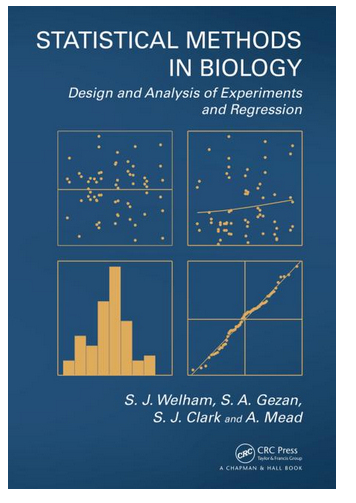
\includegraphics[width=0.3\textwidth]{welham}
\end{frame}


%%%%%%%%%%%%%%%%%%%%%%%%%%%%%%%%%%%%%%%%%%%%%%%%%%%%%%%%%%%%%%%%%%%%%%%%%%%%%%%%%%%%%%%%%%%%%%%%%%%
% Slide
%%%%%%%%%%%%%%%%%%%%%%%%%%%%%%%%%%%%%%%%%%%%%%%%%%%%%%%%%%%%%%%%%%%%%%%%%%%%%%%%%%%%%%%%%%%%%%%%%%%
\begin{frame} \frametitle{Overview}
\begin{itemize}
\item Introduction
\item Linear models - Analysis of Variance
\begin{itemize}
\item Completely Randomised Design
\item Randomised Complete Block Design
\item Latin Square
\item Factorial Treatment Structures
\end{itemize}
\item Linear Mixed Models
\begin{itemize}
\item Split-plot Design
\item Spatial Analysis
\item Complex Treatment Structures
\end{itemize}
\end{itemize}

\end{frame}

%%%%%%%%%%%%%%%%%%%%%%%%%%%%%%%%%%%%%%%%%%%%%%%%%%%%%%%%%%%%%%%%%%%%%%%%%%%%%%%%%%%%%%%%%%%%%%%%%%%
% Slide
%%%%%%%%%%%%%%%%%%%%%%%%%%%%%%%%%%%%%%%%%%%%%%%%%%%%%%%%%%%%%%%%%%%%%%%%%%%%%%%%%%%%%%%%%%%%%%%%%%%
\section{Introduction}
\begin{frame}\frametitle{Data Analysis - A Cyclical Process}
Data analysis is an important part of the scientific process and can be done by following a process but it is really
crucial you examine all the results in the context of the analysis. As a result the data analysis process is not a
linear process but a cyclical one. We will discuss this through the workshop but first we will explore the different
types of analysis covered in this workshop.

\vspace{1cm}
\centering
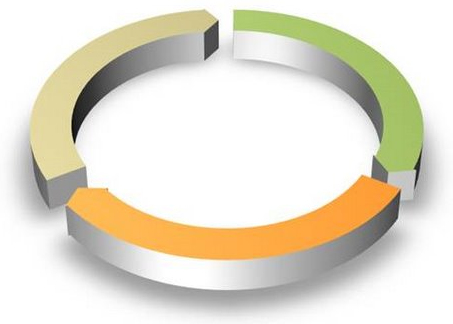
\includegraphics[width=0.3\textwidth]{cyclical}
\end{frame}

%%%%%%%%%%%%%%%%%%%%%%%%%%%%%%%%%%%%%%%%%%%%%%%%%%%%%%%%%%%%%%%%%%%%%%%%%%%%%%%%%%%%%%%%%%%%%%%%%%%
% Slide
%%%%%%%%%%%%%%%%%%%%%%%%%%%%%%%%%%%%%%%%%%%%%%%%%%%%%%%%%%%%%%%%%%%%%%%%%%%%%%%%%%%%%%%%%%%%%%%%%%%
\begin{frame}\frametitle{Types of Analyses}
The type of analysis required depends on:

\begin{enumerate}
\item the aim of the analysis (exploring relationships or the effect of a treatment or some other aim)
\item the type of data of the response variable (quantitative or qualitative)
\item the type of data of the explanatory variable/s (quantitative and/or qualitative)
\item the design of the experiment
\item \textcolor[rgb]{0.00,0.74,0.74}{whether the model assumptions are met}
\end{enumerate}

\end{frame}


%%%%%%%%%%%%%%%%%%%%%%%%%%%%%%%%%%%%%%%%%%%%%%%%%%%%%%%%%%%%%%%%%%%%%%%%%%%%%%%%%%%%%%%%%%%%%%%%%%%
% Slide
%%%%%%%%%%%%%%%%%%%%%%%%%%%%%%%%%%%%%%%%%%%%%%%%%%%%%%%%%%%%%%%%%%%%%%%%%%%%%%%%%%%%%%%%%%%%%%%%%%%
\begin{frame}\frametitle{Analysis Decision Tree}
\centering
\includegraphics[width = 0.7\textwidth]{LMFlowChart}
\end{frame}

%%%%%%%%%%%%%%%%%%%%%%%%%%%%%%%%%%%%%%%%%%%%%%%%%%%%%%%%%%%%%%%%%%%%%%%%%%%%%%%%%%%%%%%%%%%%%%%%%%%
% Slide
%%%%%%%%%%%%%%%%%%%%%%%%%%%%%%%%%%%%%%%%%%%%%%%%%%%%%%%%%%%%%%%%%%%%%%%%%%%%%%%%%%%%%%%%%%%%%%%%%%%
\begin{frame}\frametitle{Data Types}
\centering
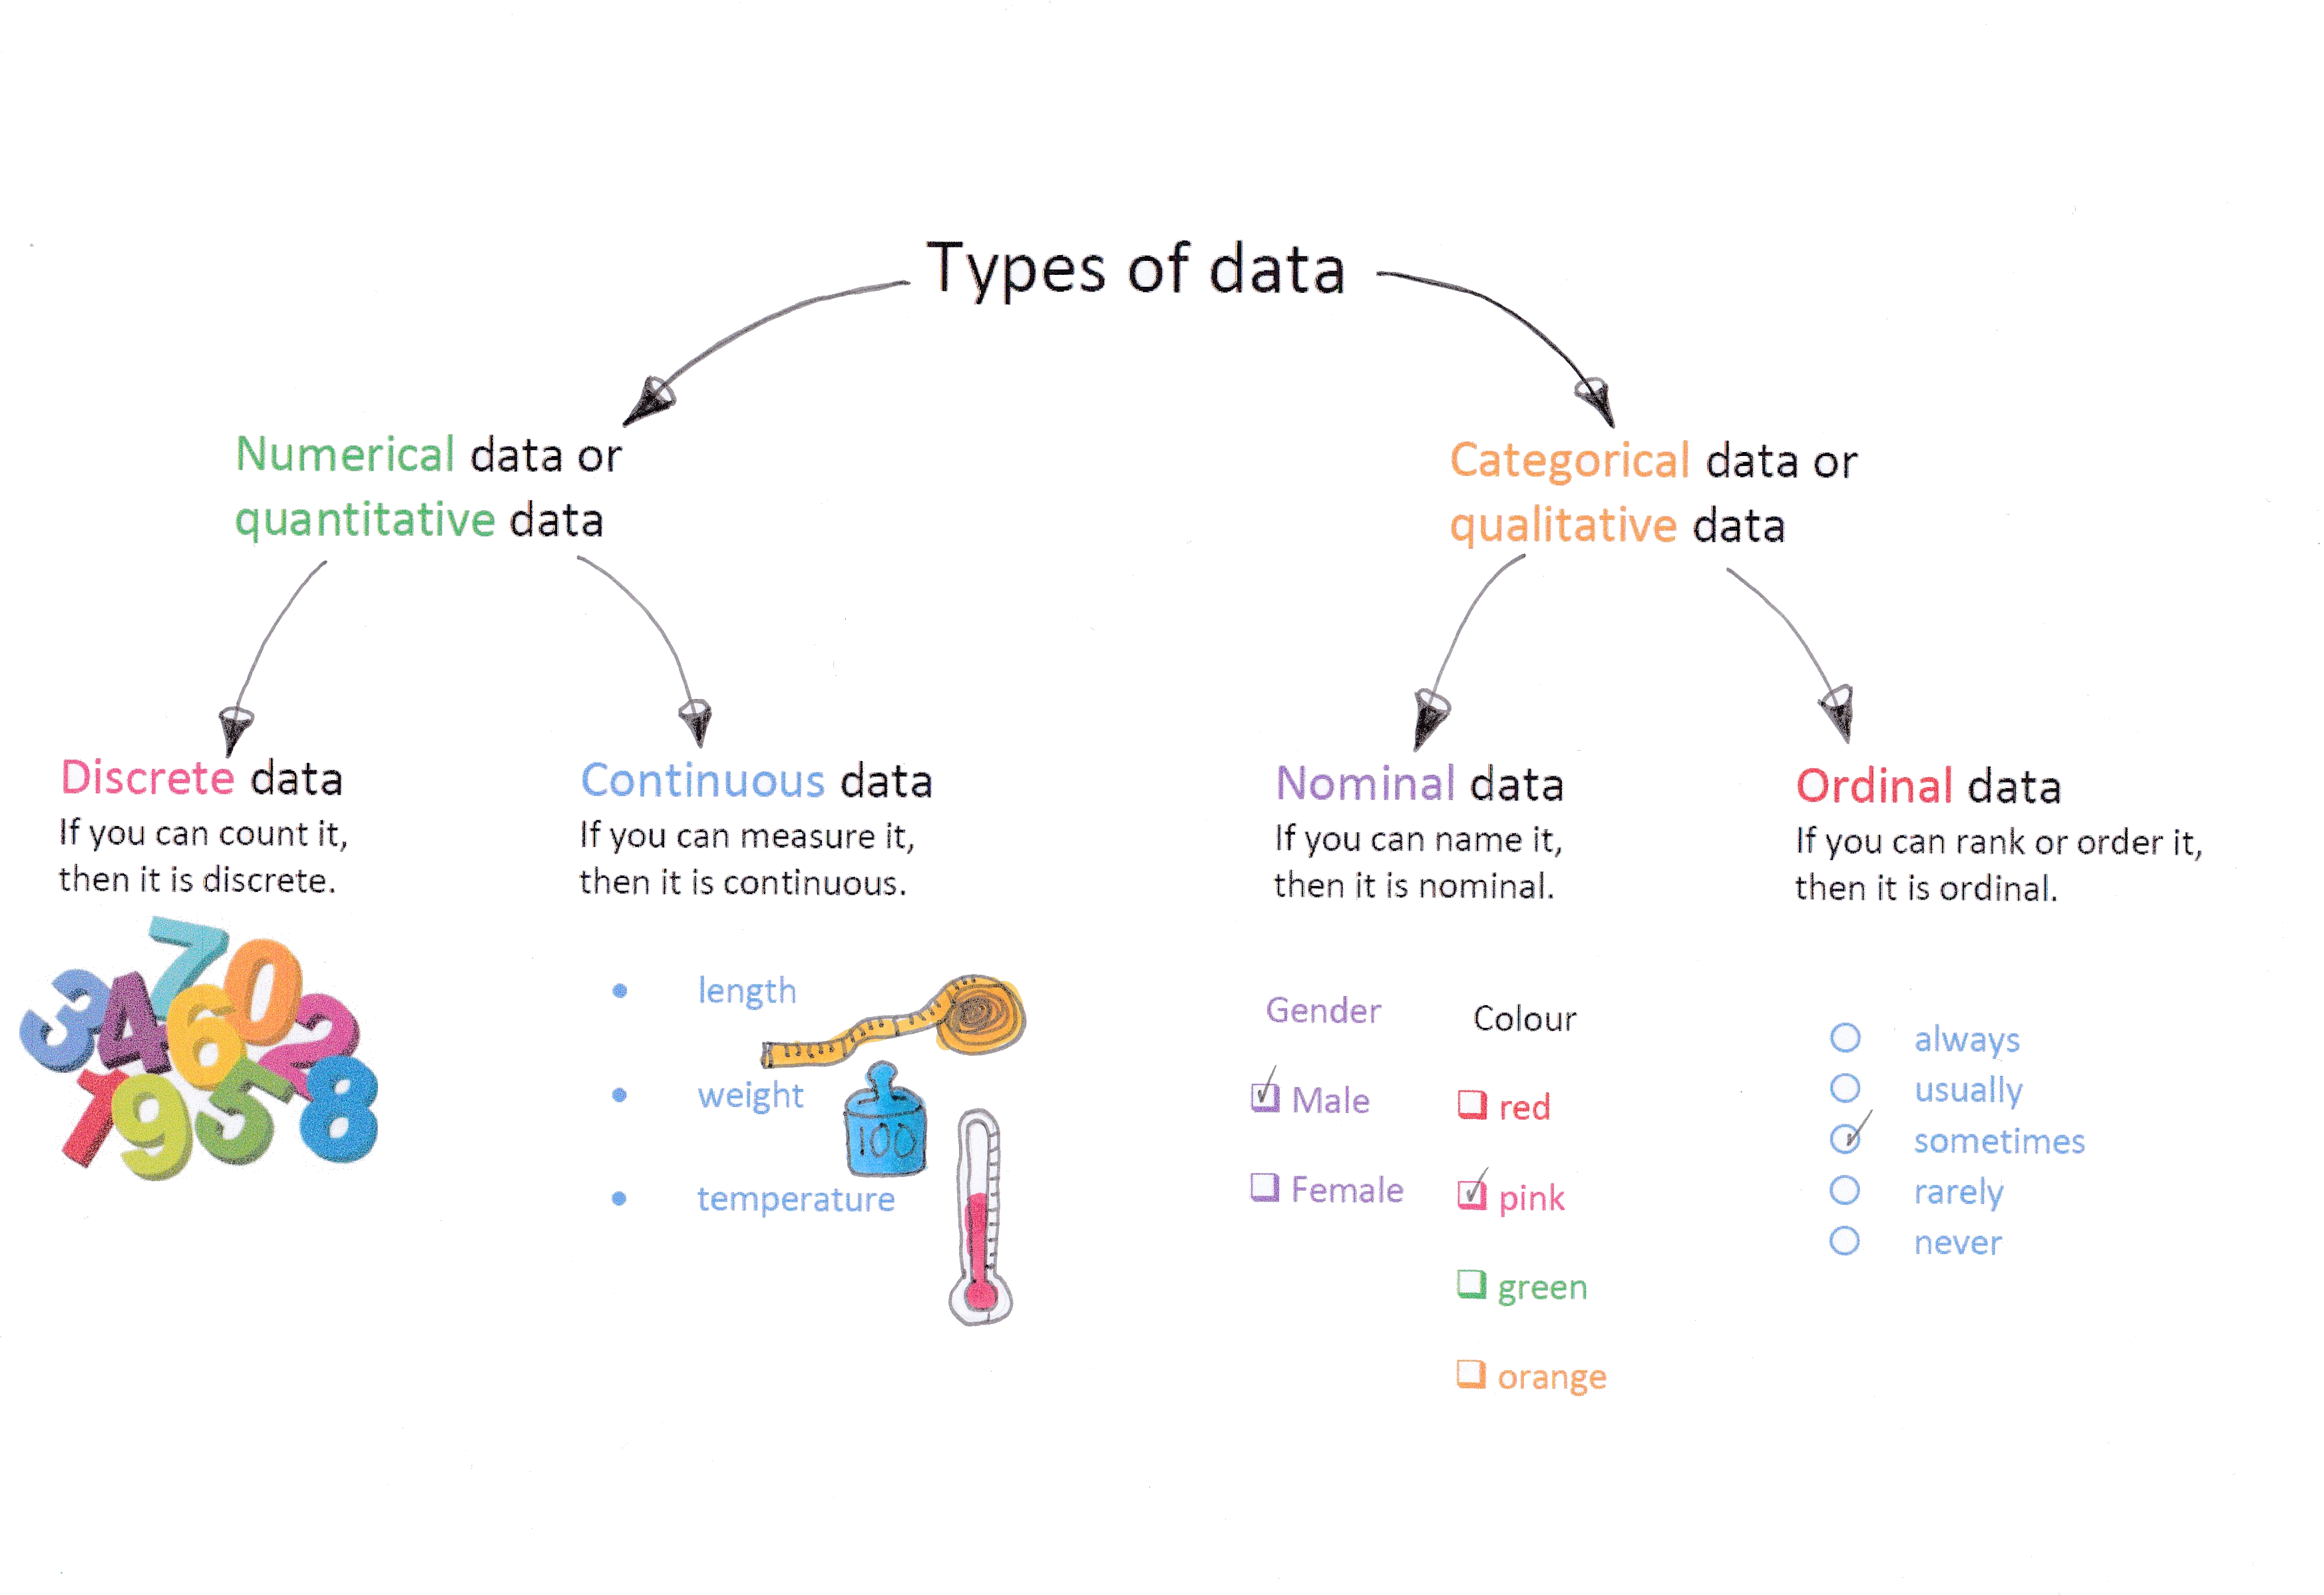
\includegraphics[width = 0.85\textwidth]{datatypes}
\end{frame}

%%%%%%%%%%%%%%%%%%%%%%%%%%%%%%%%%%%%%%%%%%%%%%%%%%%%%%%%%%%%%%%%%%%%%%%%%%%%%%%%%%%%%%%%%%%%%%%%%%%
% Slide
%%%%%%%%%%%%%%%%%%%%%%%%%%%%%%%%%%%%%%%%%%%%%%%%%%%%%%%%%%%%%%%%%%%%%%%%%%%%%%%%%%%%%%%%%%%%%%%%%%%
\begin{frame}\frametitle{Data Types}
\tiny
\begin{table}[!hbp]
\begin{tabular}{|c|l|l|l|}
  \hline
  \textbf{Data} & \textbf{Example} & \textbf{Graphical} & \textbf{Statistical} \\
  \textbf{Type} & & \textbf{Techniques} & \textbf{Model} \\
  \hline
  \multirow{13}{*}{\rotatebox{90}{Discrete}} & \textbf{Counts - } & Column  & Generalised Linear Models  \\
           & faecal egg count  & or bar chart  & (GLM) with a Poisson \\
           & number of cells  &   &  distribution  \\
           & number of species  &  &  \\
  \cline{2-4}
           & \textbf{Scores - } &  Column & Sometimes analysed as \\
           & lodging &  or bar chart    & normal continuous data \\
           & disease score &  & ANOVA$^\ast$, linear models \\
           & zadoks &  & - but this might not be \\
           & &  & appropriate \\
  \cline{2-4}
           & \textbf{Categorical -}  &  Column & GLM - for example:   \\
           & dead/alive  &  or bar chart & logistic regression  \\
           & colour (red/blue/green)  &  &    \\
           & low/medium/high  &  &    \\
\hline
 \multirow{6}{*}{\rotatebox{90}{Continuous}} & \textbf{Measurements - } & Histogram & Linear models$^\ast$, including: \\
    & pH &  or Box plot & Simple Linear Regression\\
    & temperature & & Multiple Linear Regression\\
    & weight & & Polynomial Regression\\
    & height & & Analysis of Variance (ANOVA)\\
    & \% & & Analysis of Covariance\\
 \hline
    \multicolumn{4}{|c|}{$^\ast$  Transformations may be required to meet model assumptions}\\
 \hline
\end{tabular}
\end{table}
\end{frame}

%%%%%%%%%%%%%%%%%%%%%%%%%%%%%%%%%%%%%%%%%%%%%%%%%%%%%%%%%%%%%%%%%%%%%%%%%%%%%%%%%%%%%%%%%%%%%%%%%%%
% Slide
%%%%%%%%%%%%%%%%%%%%%%%%%%%%%%%%%%%%%%%%%%%%%%%%%%%%%%%%%%%%%%%%%%%%%%%%%%%%%%%%%%%%%%%%%%%%%%%%%%%
\begin{frame}\frametitle{Commonly used designs}
The designs studied in W1 Planning and Designing Agronomic Experiments were:

\begin{itemize}
\item Completely Randomised Design (CRD)
\item Randomised Complete Block Design (RCBD)
\item Latin Square
\item Factorial Treatment Structures
\item Split-plot
\end{itemize}

In this workshop we will consider the analysis of these experiments using the R statistical package \cite{r}.

\end{frame}


\section{Linear models - Analysis of Variance}
\subsection{Completely Randomised Design}
%%%%%%%%%%%%%%%%%%%%%%%%%%%%%%%%%%%%%%%%%%%%%%%%%%%%%%%%%%%%%%%%%%%%%%%%%%%%%%%%%%%%%%%%%%%%%%%%%%%
% Slide
%%%%%%%%%%%%%%%%%%%%%%%%%%%%%%%%%%%%%%%%%%%%%%%%%%%%%%%%%%%%%%%%%%%%%%%%%%%%%%%%%%%%%%%%%%%%%%%%%%%
\begin{frame}\frametitle{Completely Randomised Design (CRD)}
In a CRD the random allocation of treatments to experimental units is not constrained in any way. Usually the aim of
the analysis of this type of experiment is to determine whether treatment differences exist. The usual hypothesis test
is
\begin{eqnarray*}
	H_0&:& \mu_1 = \mu_2 = \hdots = \mu_t \\
	H_1&:& \texttt{not all treatment means are the same}
\end{eqnarray*}

\end{frame}



%%%%%%%%%%%%%%%%%%%%%%%%%%%%%%%%%%%%%%%%%%%%%%%%%%%%%%%%%%%%%%%%%%%%%%%%%%%%%%%%%%%%%%%%%%%%%%%%%%%
% Slide
%%%%%%%%%%%%%%%%%%%%%%%%%%%%%%%%%%%%%%%%%%%%%%%%%%%%%%%%%%%%%%%%%%%%%%%%%%%%%%%%%%%%%%%%%%%%%%%%%%
\begin{frame}\frametitle{CRD}
\begin{columns}
\begin{column}{0.5\textwidth}
\centering
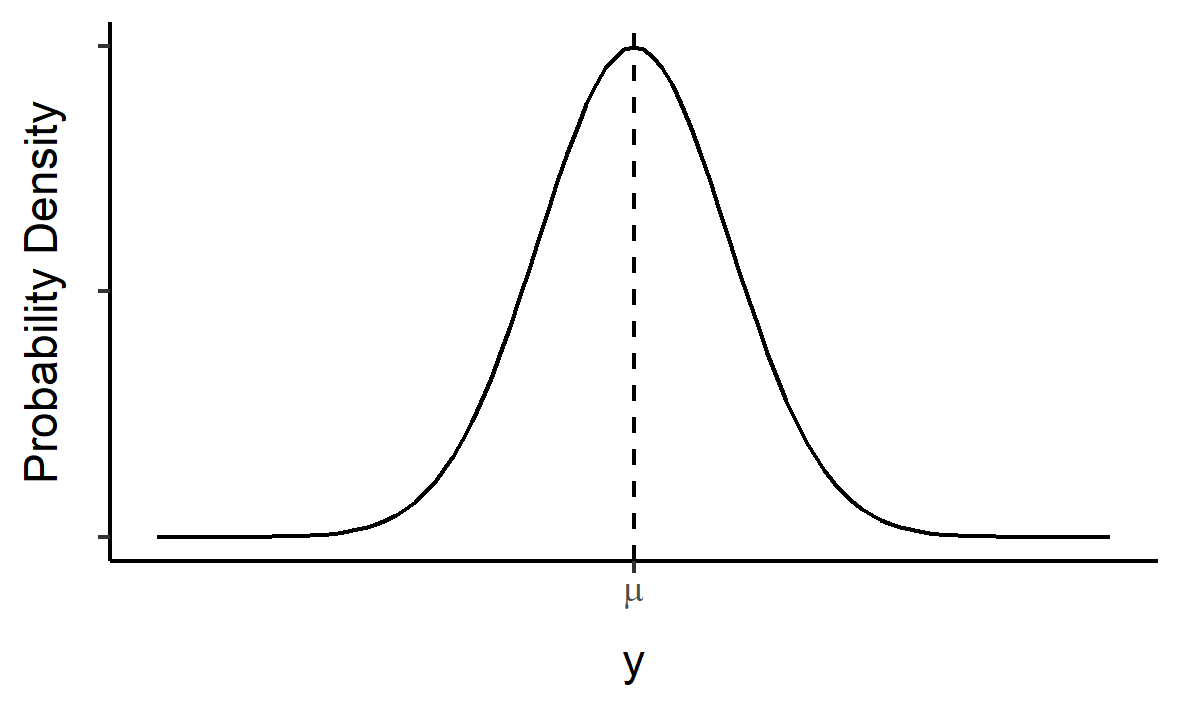
\includegraphics[width = \textwidth]{CRDnullNormDensity.png}
\end{column}
\begin{column}{0.5\textwidth}
\centering
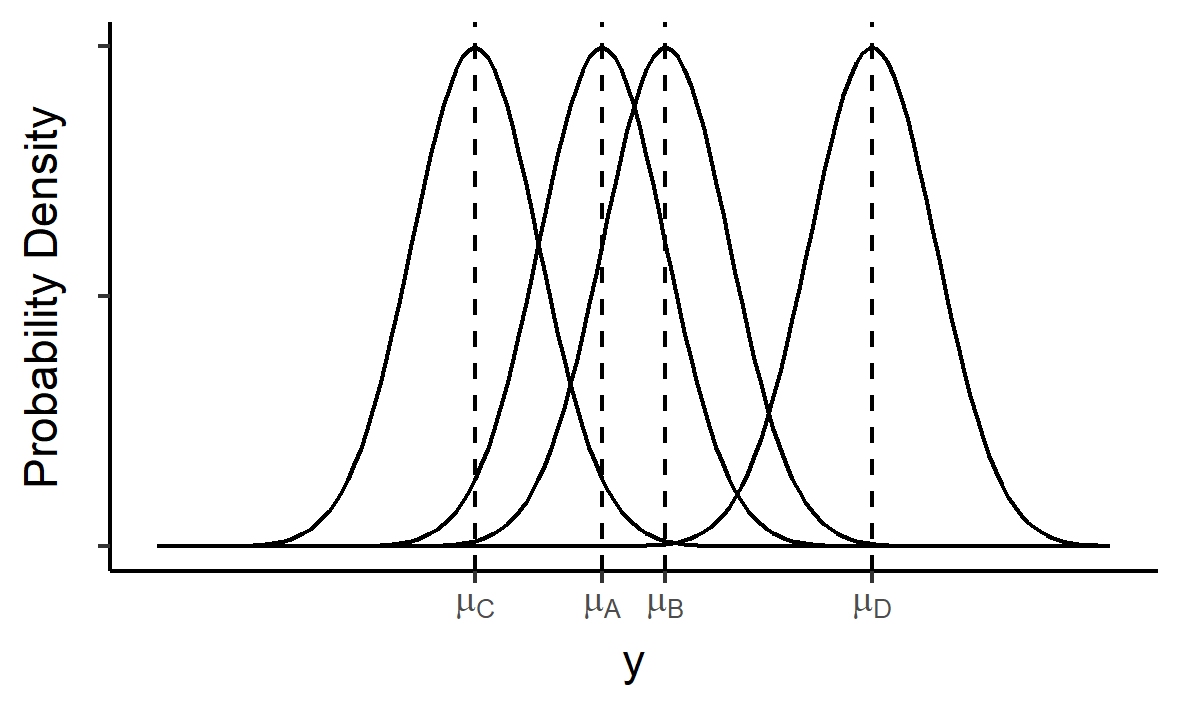
\includegraphics[width = \textwidth]{CRDAlternativeNormDensity.png}
\end{column}
\end{columns}


\vspace{1cm}
\flushright

\includegraphics[height = 0.3cm]{yourturn}
\end{frame}


%%%%%%%%%%%%%%%%%%%%%%%%%%%%%%%%%%%%%%%%%%%%%%%%%%%%%%%%%%%%%%%%%%%%%%%%%%%%%%%%%%%%%%%%%%%%%%%%%%%
% Slide
%%%%%%%%%%%%%%%%%%%%%%%%%%%%%%%%%%%%%%%%%%%%%%%%%%%%%%%%%%%%%%%%%%%%%%%%%%%%%%%%%%%%%%%%%%%%%%%%%%%
\begin{frame}[fragile]\frametitle{CRD ANOVA}
The aim of Analysis of variance is to partition the variance of the response up into two or more parts. From the design
course we know that the skeletal ANOVA table for a CRD looks like:

\begin{verbatim}
Source of Variation                      df
=============================================
Treatment                                t-1
Residual                                 n-t
=============================================
Total                                    n-1
\end{verbatim}

where $t$ are the number of treatments and $n$ is the total number of responses. This ANOVA table shows that for a CRD
the variance is partitioned up into the variance that is associated with the treatments and the variance that is
associated with the residual or unexplained variance.
\end{frame}

%%%%%%%%%%%%%%%%%%%%%%%%%%%%%%%%%%%%%%%%%%%%%%%%%%%%%%%%%%%%%%%%%%%%%%%%%%%%%%%%%%%%%%%%%%%%%%%%%%%
% Slide
%%%%%%%%%%%%%%%%%%%%%%%%%%%%%%%%%%%%%%%%%%%%%%%%%%%%%%%%%%%%%%%%%%%%%%%%%%%%%%%%%%%%%%%%%%%%%%%%%%%
\begin{frame}\frametitle{CRD ANOVA}
\centering
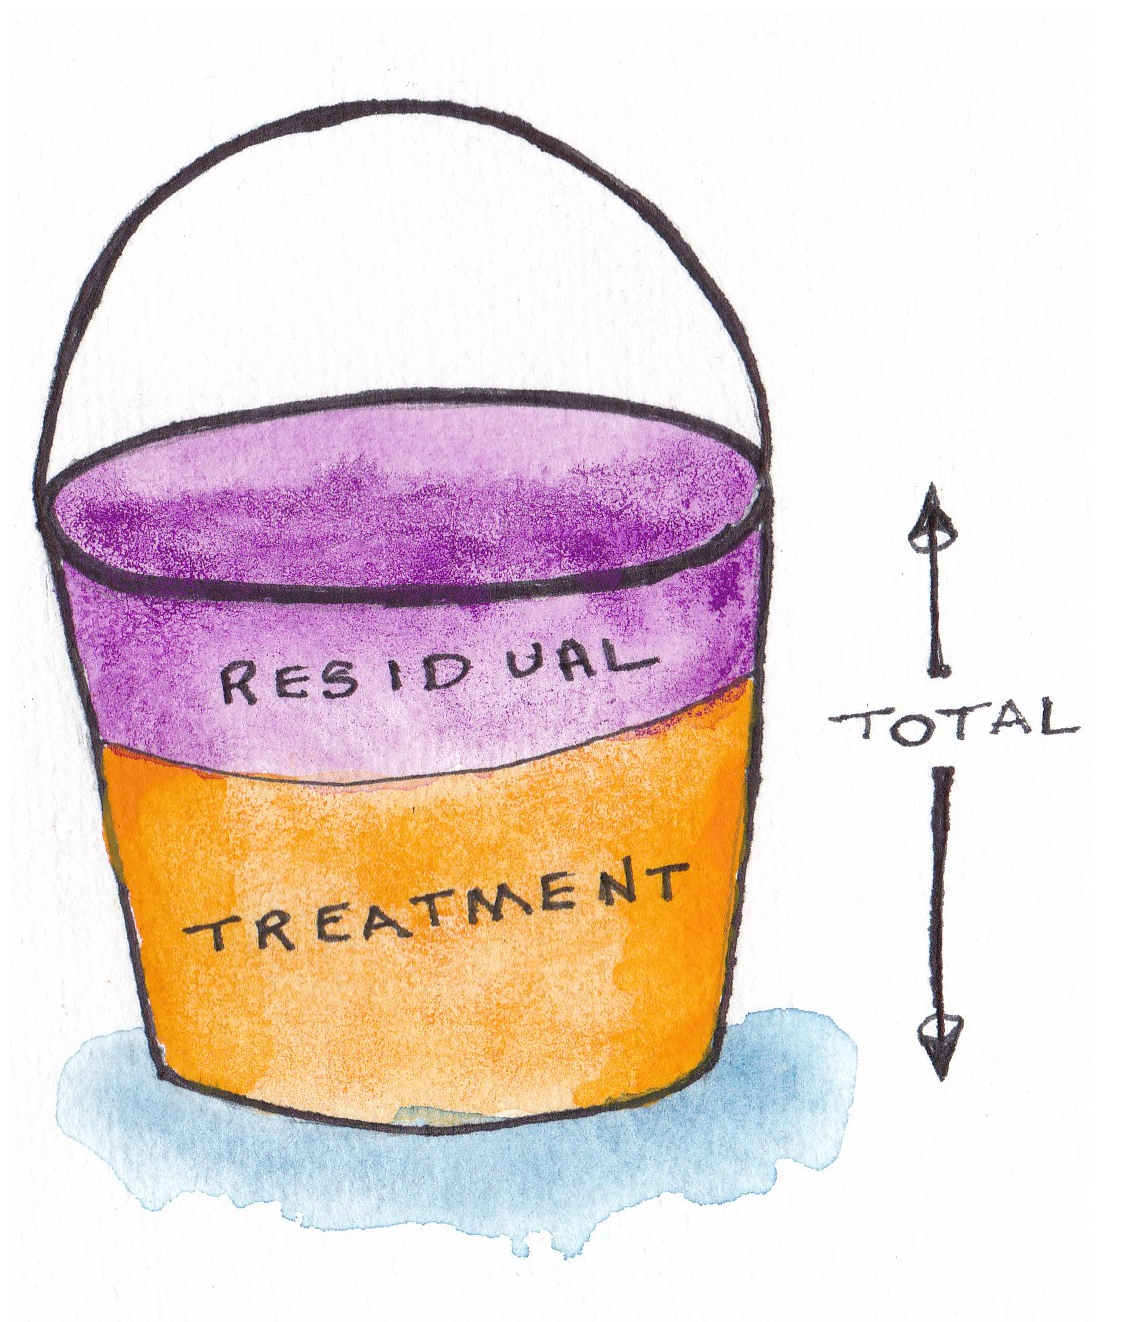
\includegraphics[width = 0.4\textwidth]{crdbucket.png}
\end{frame}


%%%%%%%%%%%%%%%%%%%%%%%%%%%%%%%%%%%%%%%%%%%%%%%%%%%%%%%%%%%%%%%%%%%%%%%%%%%%%%%%%%%%%%%%%%%%%%%%%%%
% Slide
%%%%%%%%%%%%%%%%%%%%%%%%%%%%%%%%%%%%%%%%%%%%%%%%%%%%%%%%%%%%%%%%%%%%%%%%%%%%%%%%%%%%%%%%%%%%%%%%%%%
\begin{frame}\frametitle{Hypothetical CRD}
Completely randomised design with three treatments and four replicates.

\begin{table}[ht]
\centering
\begin{tabular}{cc}
 \toprule
  treatment & response \\
  \midrule
  A & 4.28 \\
  A & 4.04 \\
  A & 4.67 \\
  A & 3.11 \\
  B & 6.29 \\
  B & 5.90 \\
  B & 7.21 \\
  B & 8.60 \\
  C & 6.17 \\
   C & 5.42 \\
   C & 5.85 \\
   C & 7.77 \\
   \bottomrule
\end{tabular}
\end{table}

\end{frame}



%%%%%%%%%%%%%%%%%%%%%%%%%%%%%%%%%%%%%%%%%%%%%%%%%%%%%%%%%%%%%%%%%%%%%%%%%%%%%%%%%%%%%%%%%%%%%%%%%%%
% Slide
%%%%%%%%%%%%%%%%%%%%%%%%%%%%%%%%%%%%%%%%%%%%%%%%%%%%%%%%%%%%%%%%%%%%%%%%%%%%%%%%%%%%%%%%%%%%%%%%%%%
\begin{frame}\frametitle{Hypothetical CRD}
\centering
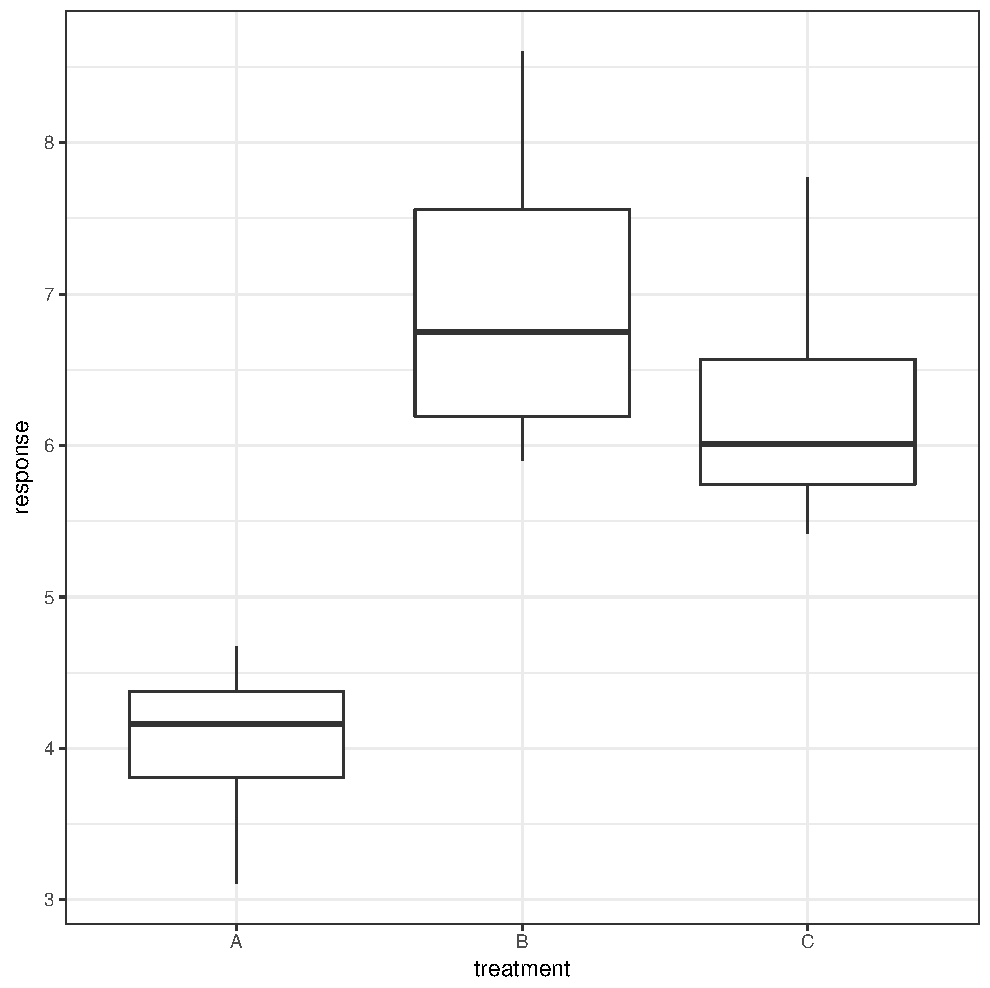
\includegraphics[width=0.5\textwidth]{hypcrd_boxplot.pdf}
\end{frame}

%%%%%%%%%%%%%%%%%%%%%%%%%%%%%%%%%%%%%%%%%%%%%%%%%%%%%%%%%%%%%%%%%%%%%%%%%%%%%%%%%%%%%%%%%%%%%%%%%%%
% Slide
%%%%%%%%%%%%%%%%%%%%%%%%%%%%%%%%%%%%%%%%%%%%%%%%%%%%%%%%%%%%%%%%%%%%%%%%%%%%%%%%%%%%%%%%%%%%%%%%%%%
\begin{frame}\frametitle{Hypothetical CRD}
\centering
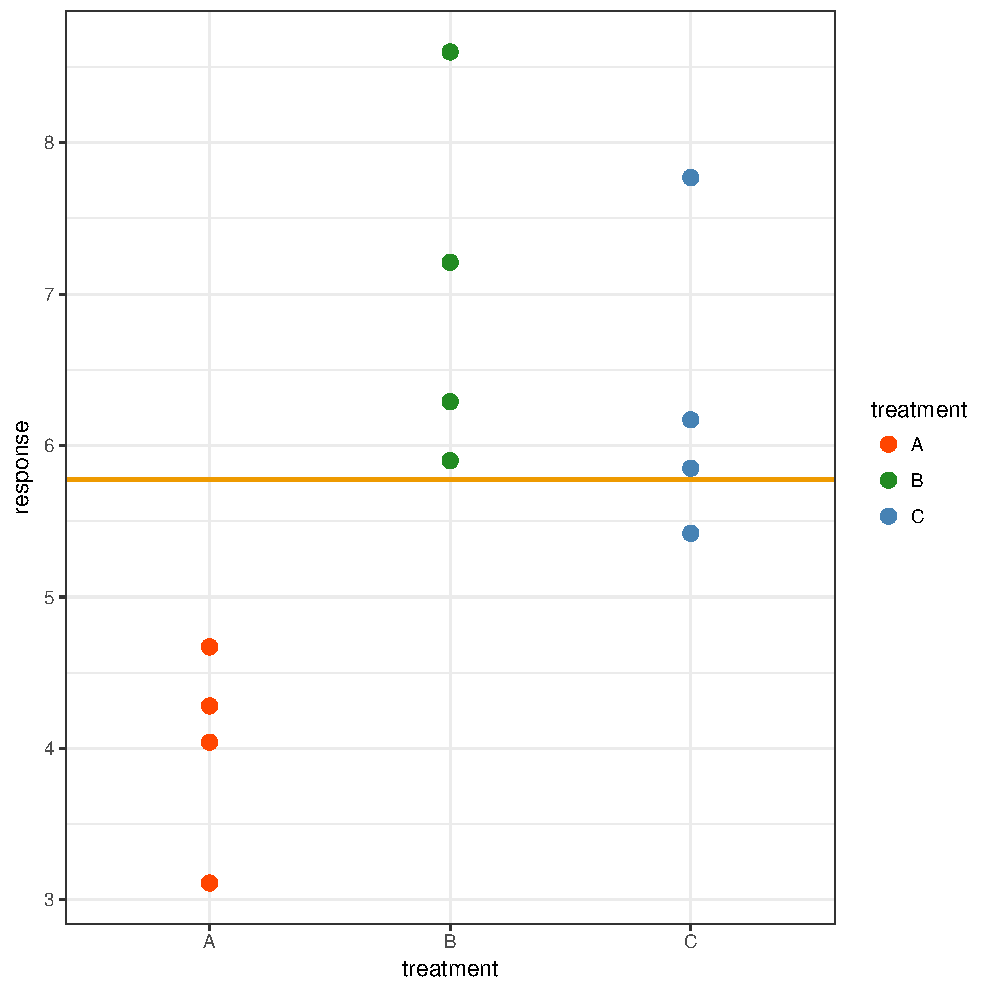
\includegraphics[width=0.5\textwidth]{hypcrd_overallmean.pdf}
\end{frame}

%%%%%%%%%%%%%%%%%%%%%%%%%%%%%%%%%%%%%%%%%%%%%%%%%%%%%%%%%%%%%%%%%%%%%%%%%%%%%%%%%%%%%%%%%%%%%%%%%%%
% Slide
%%%%%%%%%%%%%%%%%%%%%%%%%%%%%%%%%%%%%%%%%%%%%%%%%%%%%%%%%%%%%%%%%%%%%%%%%%%%%%%%%%%%%%%%%%%%%%%%%%%
\begin{frame}\frametitle{Hypothetical CRD}
\centering
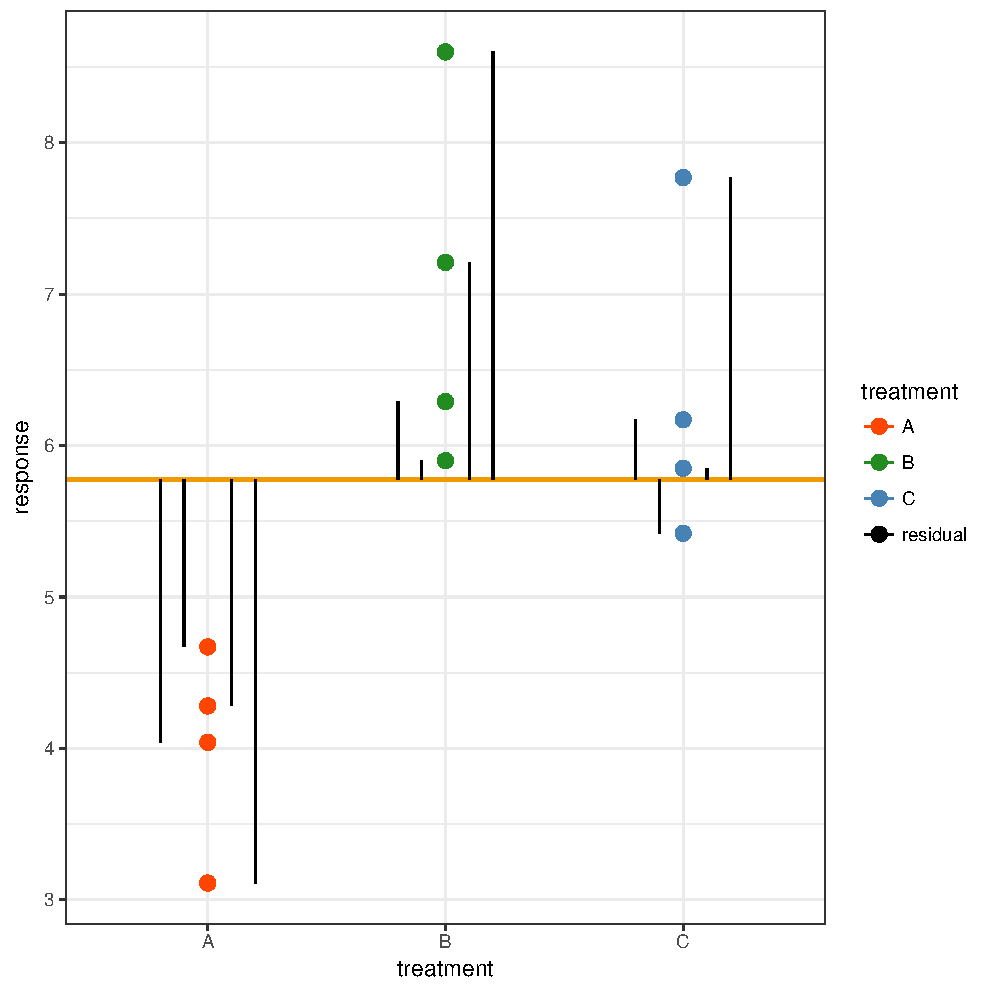
\includegraphics[width=0.5\textwidth]{hypcrd_totss.pdf}
\end{frame}


%%%%%%%%%%%%%%%%%%%%%%%%%%%%%%%%%%%%%%%%%%%%%%%%%%%%%%%%%%%%%%%%%%%%%%%%%%%%%%%%%%%%%%%%%%%%%%%%%%%
% Slide
%%%%%%%%%%%%%%%%%%%%%%%%%%%%%%%%%%%%%%%%%%%%%%%%%%%%%%%%%%%%%%%%%%%%%%%%%%%%%%%%%%%%%%%%%%%%%%%%%%%
\begin{frame}\frametitle{Hypothetical CRD}
\centering
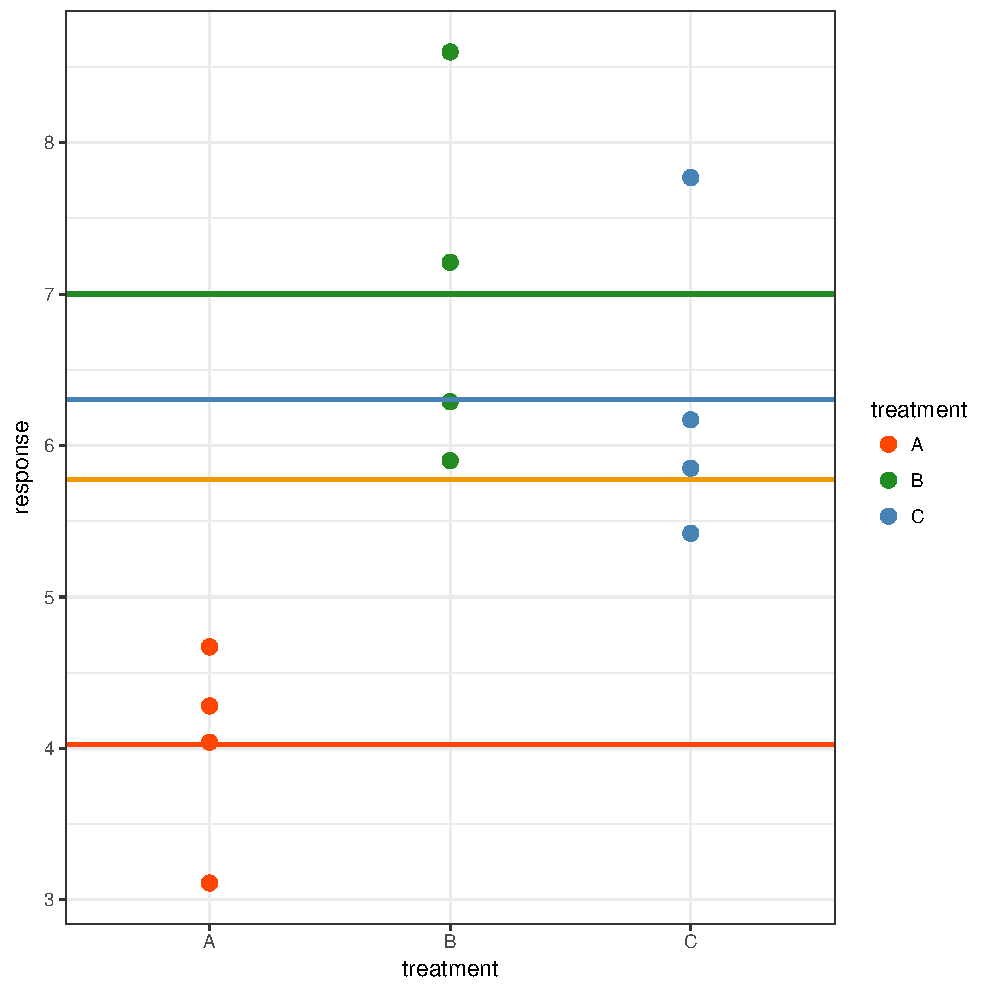
\includegraphics[width=0.5\textwidth]{hypcrd_trtmean.pdf}
\end{frame}

%%%%%%%%%%%%%%%%%%%%%%%%%%%%%%%%%%%%%%%%%%%%%%%%%%%%%%%%%%%%%%%%%%%%%%%%%%%%%%%%%%%%%%%%%%%%%%%%%%%
% Slide
%%%%%%%%%%%%%%%%%%%%%%%%%%%%%%%%%%%%%%%%%%%%%%%%%%%%%%%%%%%%%%%%%%%%%%%%%%%%%%%%%%%%%%%%%%%%%%%%%%%
\begin{frame}\frametitle{Hypothetical CRD}
\centering
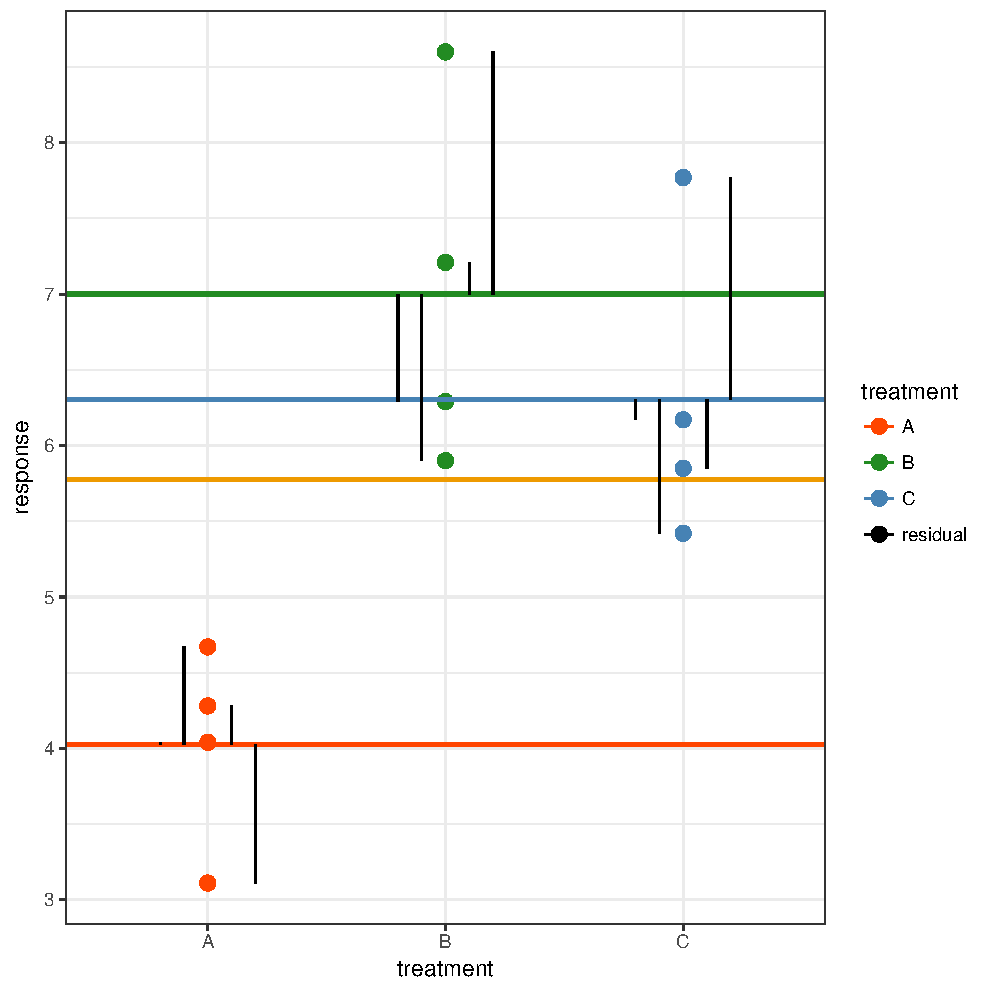
\includegraphics[width=0.5\textwidth]{hypcrd_trtss.pdf}
\end{frame}


%%%%%%%%%%%%%%%%%%%%%%%%%%%%%%%%%%%%%%%%%%%%%%%%%%%%%%%%%%%%%%%%%%%%%%%%%%%%%%%%%%%%%%%%%%%%%%%%%%%
% Slide
%%%%%%%%%%%%%%%%%%%%%%%%%%%%%%%%%%%%%%%%%%%%%%%%%%%%%%%%%%%%%%%%%%%%%%%%%%%%%%%%%%%%%%%%%%%%%%%%%%%
\begin{frame}\frametitle{Means and Effects}

The distance from the overall mean to the treatment mean is called the \textbf{effect} of the treatment. An
effect is the difference between two means.
\vspace{1cm}


\begin{center}
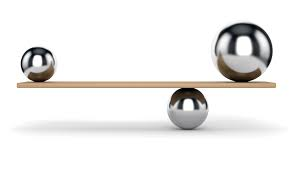
\includegraphics[width=0.4\textwidth]{effects.jpg}
\end{center}
\end{frame}


%%%%%%%%%%%%%%%%%%%%%%%%%%%%%%%%%%%%%%%%%%%%%%%%%%%%%%%%%%%%%%%%%%%%%%%%%%%%%%%%%%%%%%%%%%%%%%%%%%%
% Slide
%%%%%%%%%%%%%%%%%%%%%%%%%%%%%%%%%%%%%%%%%%%%%%%%%%%%%%%%%%%%%%%%%%%%%%%%%%%%%%%%%%%%%%%%%%%%%%%%%%%
\begin{frame}\frametitle{CRD ANOVA Table}
\begin{table}[ht]
\centering
\begin{tabular}{llllc}
\toprule
   & & & &\\
  Source & SS & df & MS & F \\
   & & & &\\
\midrule
   Treatment & $\sum\limits_{i=1}^{t}n_i(\bar{y}_{i}-\bar{y})^2$ & $t-1$ & $\frac{SS_{Trt}}{df_{Trt}}$ & $\frac{MS_{Trt}}{MS_{Residual}}$ \\
   & & & &\\
  Residual & $\sum\limits_{i=1}^{t} \sum\limits_{j=1}^{r} (y_{ij}-\bar{y}_{i})^2$ & $\sum\limits_{i=1}^{t}(n_i-t)$ & $\frac{SS_{Residual}}{df_{Residual}}$ &  \\
   & & & &\\
   Total & $\sum\limits_{i=1}^{t} \sum\limits_{j=1}^{r} (y_{ij}-\bar{y})^2 $ & $\sum\limits_{i=1}^{t}(n_i-1)$ &  &  \\
   & & & &\\
\bottomrule
\end{tabular}
\end{table}

\end{frame}


%%%%%%%%%%%%%%%%%%%%%%%%%%%%%%%%%%%%%%%%%%%%%%%%%%%%%%%%%%%%%%%%%%%%%%%%%%%%%%%%%%%%%%%%%%%%%%%%%%%
% Slide
%%%%%%%%%%%%%%%%%%%%%%%%%%%%%%%%%%%%%%%%%%%%%%%%%%%%%%%%%%%%%%%%%%%%%%%%%%%%%%%%%%%%%%%%%%%%%%%%%%%
\begin{frame}\frametitle{Partitioning under the null and alternative hypothesis}
\centering
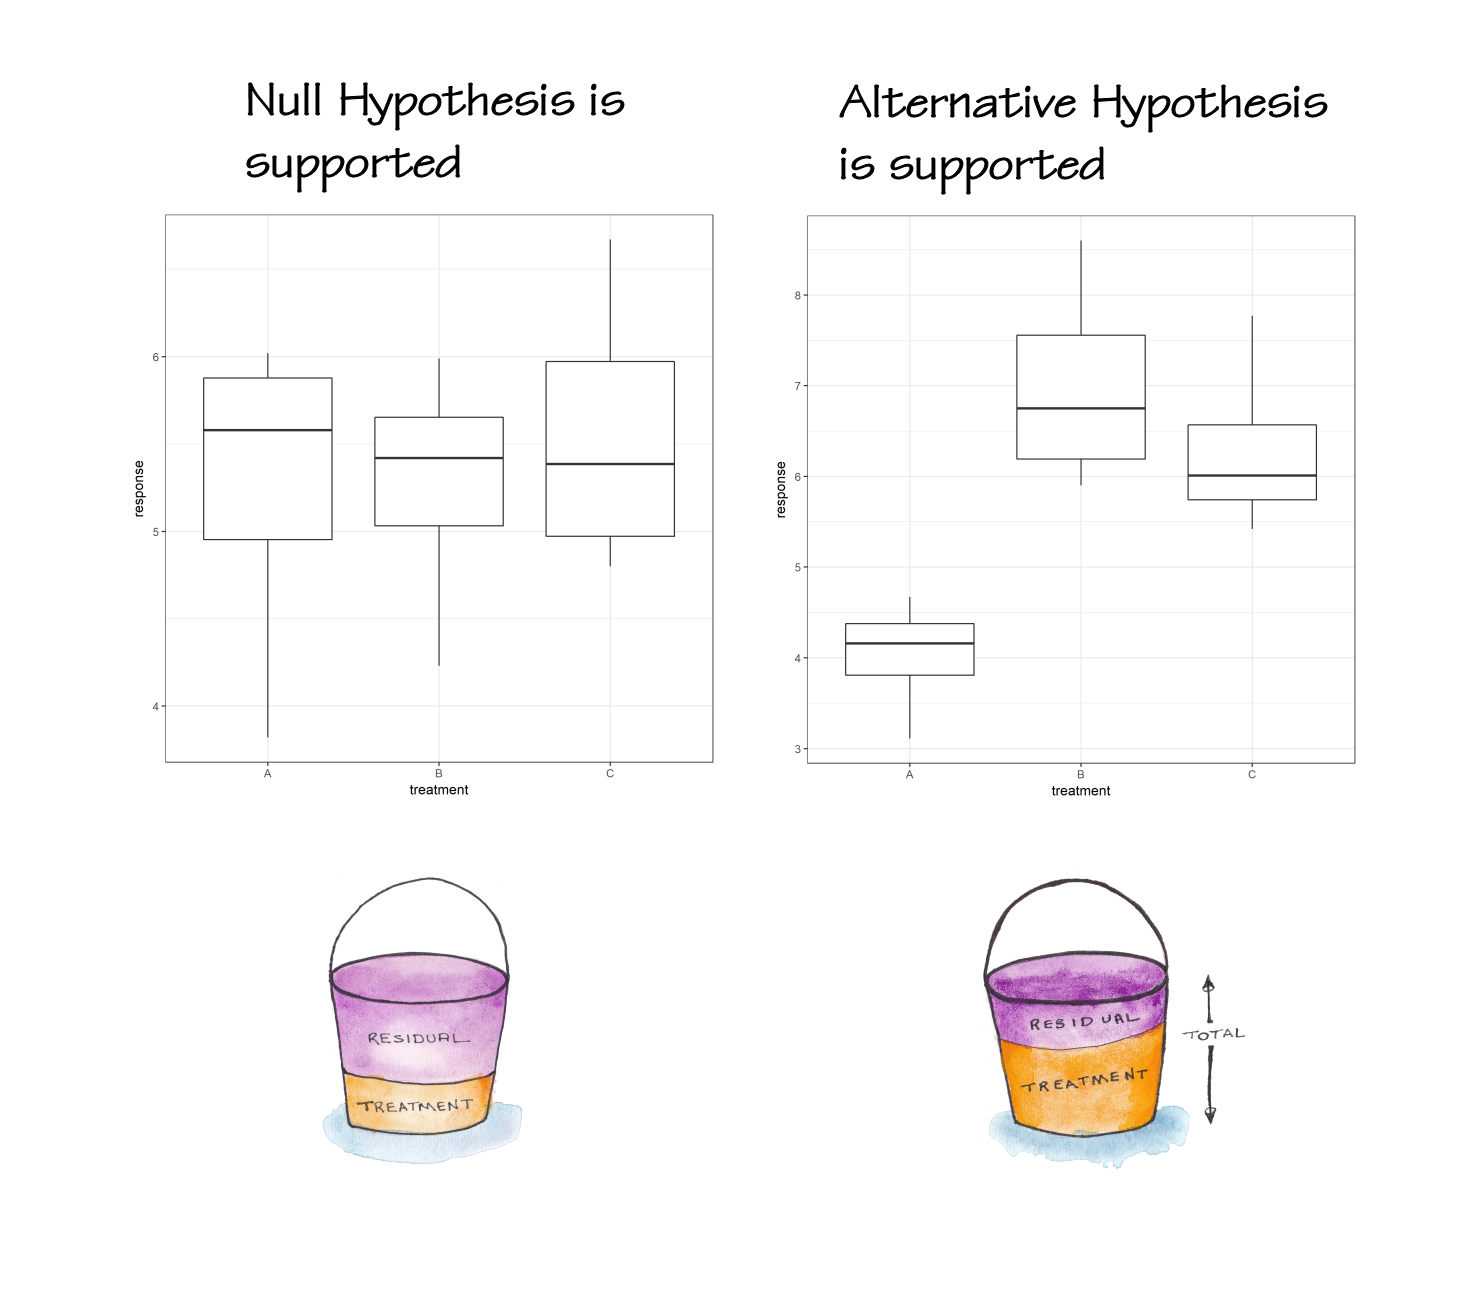
\includegraphics[height = 0.9\textheight]{compAcrd.png}
\end{frame}



%%%%%%%%%%%%%%%%%%%%%%%%%%%%%%%%%%%%%%%%%%%%%%%%%%%%%%%%%%%%%%%%%%%%%%%%%%%%%%%%%%%%%%%%%%%%%%%%%%%
% Slide
%%%%%%%%%%%%%%%%%%%%%%%%%%%%%%%%%%%%%%%%%%%%%%%%%%%%%%%%%%%%%%%%%%%%%%%%%%%%%%%%%%%%%%%%%%%%%%%%%%%
\begin{frame}\frametitle{Example 1}

An experiment was run to investigate the effect of the differences in soil calcium on the root growth of plants. The
experimental material consisted of 20 pots, each containing one plant, arranged in a rectangular array of four rows and
five columns, under uniform controlled conditions. The treatments comprised four relative concentrations of calcium -
1, 5, 10 and 20. Each treatment was applied to five pots selected at random to give a CRD design. The data can be found
in \texttt{example1.csv}.


\vspace{1cm}
\begin{center}
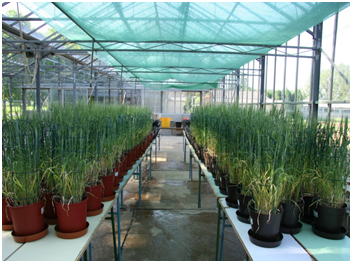
\includegraphics[height = 0.6\textheight]{glasshouse.png}
\end{center}
\end{frame}

%%%%%%%%%%%%%%%%%%%%%%%%%%%%%%%%%%%%%%%%%%%%%%%%%%%%%%%%%%%%%%%%%%%%%%%%%%%%%%%%%%%%%%%%%%%%%%%%%%%
% Slide
%%%%%%%%%%%%%%%%%%%%%%%%%%%%%%%%%%%%%%%%%%%%%%%%%%%%%%%%%%%%%%%%%%%%%%%%%%%%%%%%%%%%%%%%%%%%%%%%%%%
\begin{frame}\frametitle{Experimental Layout}

\begin{center}
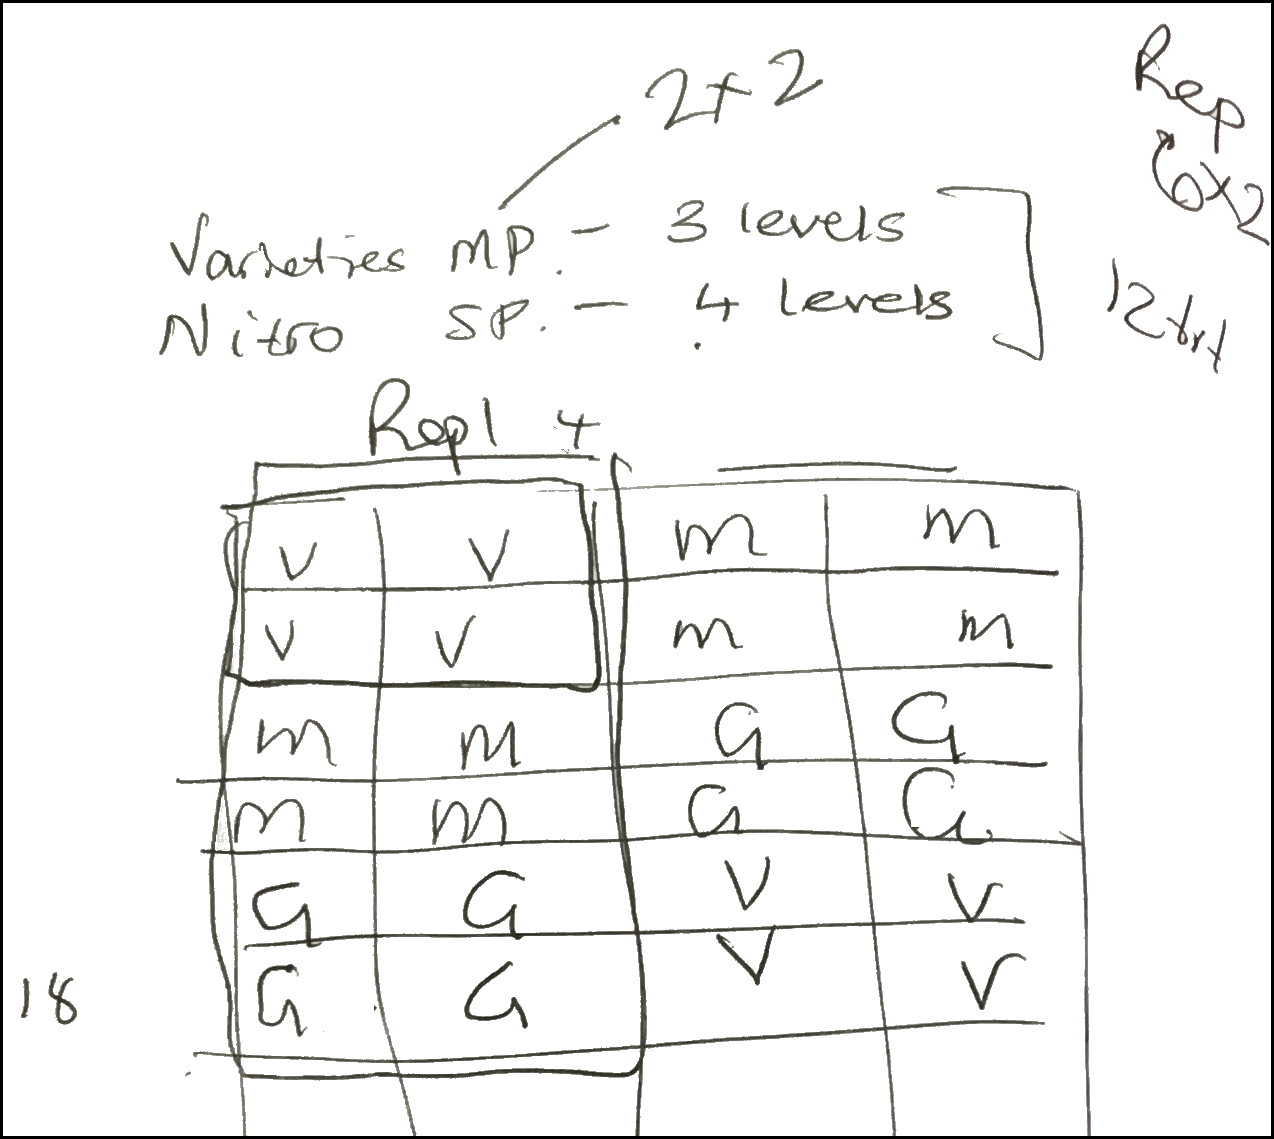
\includegraphics[height = 0.7\textheight]{exptlayout.png}
\end{center}
\flushright

\includegraphics[height = 0.3cm]{yourturn}
\end{frame}



%%%%%%%%%%%%%%%%%%%%%%%%%%%%%%%%%%%%%%%%%%%%%%%%%%%%%%%%%%%%%%%%%%%%%%%%%%%%%%%%%%%%%%%%%%%%%%%%%%%
% Slide
%%%%%%%%%%%%%%%%%%%%%%%%%%%%%%%%%%%%%%%%%%%%%%%%%%%%%%%%%%%%%%%%%%%%%%%%%%%%%%%%%%%%%%%%%%%%%%%%%%%
\begin{frame}\frametitle{Example 1}
The analysis will be undertaken to determine
\begin{eqnarray*}
	H_0&:& \mu_1 = \mu_5 = \mu_{10} = \mu_{20} \\
	H_1&:& \texttt{not all the calcium treatment means are the same}
\end{eqnarray*}

or this can be rewritten in terms of effects
\begin{eqnarray*}
	H_0&:& \alpha_1 = \alpha_5 = \alpha_{10} = \alpha_{20} = 0 \\
	H_1&:& \texttt{not all the calcium treatment effects are zero}
\end{eqnarray*}
These are identical hypotheses.
\end{frame}


%%%%%%%%%%%%%%%%%%%%%%%%%%%%%%%%%%%%%%%%%%%%%%%%%%%%%%%%%%%%%%%%%%%%%%%%%%%%%%%%%%%%%%%%%%%%%%%%%%%
% Slide
%%%%%%%%%%%%%%%%%%%%%%%%%%%%%%%%%%%%%%%%%%%%%%%%%%%%%%%%%%%%%%%%%%%%%%%%%%%%%%%%%%%%%%%%%%%%%%%%%%%
\begin{frame}\frametitle{Example 1}

The first part of any analysis like this will be to visualise the data. We need to determine whether using usual
analysis of variance methods may be appropriate and check the data for any anomalies. When testing for the effect of a
treatment, a boxplot is an appropriate graph to use. The treatments are the $x$-variable and the response (root length)
is the dependent or $y$-variable.


\vspace{3cm}
\flushright

\includegraphics[height = 0.3cm]{yourturn}

\end{frame}



%%%%%%%%%%%%%%%%%%%%%%%%%%%%%%%%%%%%%%%%%%%%%%%%%%%%%%%%%%%%%%%%%%%%%%%%%%%%%%%%%%%%%%%%%%%%%%%%%%%
% Slide
%%%%%%%%%%%%%%%%%%%%%%%%%%%%%%%%%%%%%%%%%%%%%%%%%%%%%%%%%%%%%%%%%%%%%%%%%%%%%%%%%%%%%%%%%%%%%%%%%%%
\begin{frame}\frametitle{Example 1 Boxplot}
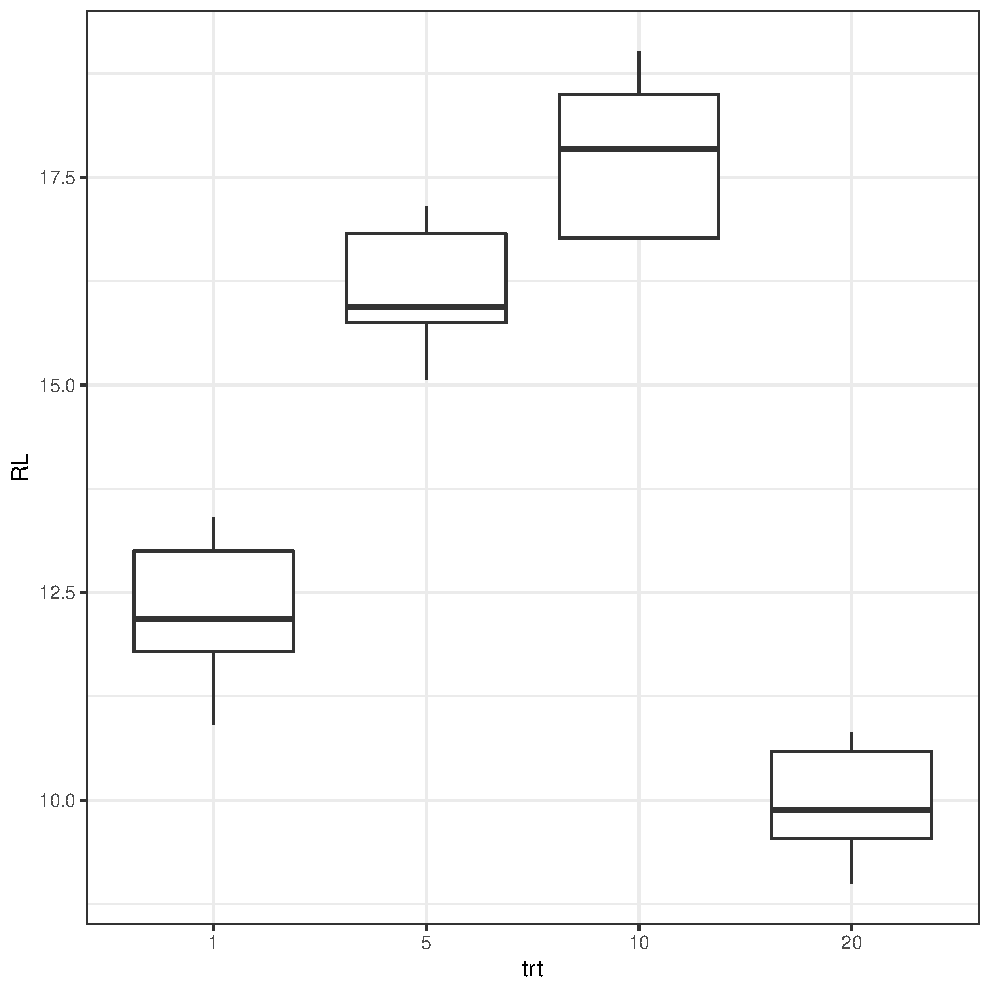
\includegraphics[width=0.5\textwidth]{example1_boxplot.pdf}
\end{frame}


%%%%%%%%%%%%%%%%%%%%%%%%%%%%%%%%%%%%%%%%%%%%%%%%%%%%%%%%%%%%%%%%%%%%%%%%%%%%%%%%%%%%%%%%%%%%%%%%%%%
% Slide
%%%%%%%%%%%%%%%%%%%%%%%%%%%%%%%%%%%%%%%%%%%%%%%%%%%%%%%%%%%%%%%%%%%%%%%%%%%%%%%%%%%%%%%%%%%%%%%%%%%
\begin{frame}\frametitle{Example 1  - Linear Model}
The linear model that is fit can be described by a simple model,

\begin{eqnarray*}
% \nonumber % Remove numbering (before each equation)
  RL_{ij} &=& \mu_i + \varepsilon_{ij}
\end{eqnarray*}

where $\mu_i$ is the true (but unknown) mean for the $i^{th}$ treatment and $\varepsilon_{ij}$ is the deviation
(residual) of the $j^{th}$ response on the $i^{th}$ treatment from its population mean.

Using symbolic notation, we can represent this equation as
\begin{eqnarray*}
	\texttt{Response variable}&:& \texttt{RL} \\
	\texttt{Explanatory component}&:& \texttt{Calcium Concentration}\\
	\texttt{Residual}&:& \texttt{Assume Independence}
\end{eqnarray*}

\end{frame}


%%%%%%%%%%%%%%%%%%%%%%%%%%%%%%%%%%%%%%%%%%%%%%%%%%%%%%%%%%%%%%%%%%%%%%%%%%%%%%%%%%%%%%%%%%%%%%%%%%%
% Slide
%%%%%%%%%%%%%%%%%%%%%%%%%%%%%%%%%%%%%%%%%%%%%%%%%%%%%%%%%%%%%%%%%%%%%%%%%%%%%%%%%%%%%%%%%%%%%%%%%%%
\begin{frame}\frametitle{Model Assumptions}
\textbf{Assumption 1}
\begin{eqnarray*}
E(\varepsilon_{ij}) = 0
\end{eqnarray*}

This means that the population mean of the residuals is zero, which implies no systematic bias in the observations.

\textbf{Assumption 2}
\begin{eqnarray*}
Var(\varepsilon_{ij}) = \sigma^2
\end{eqnarray*}

The variances of the residuals are the same for all units. This is also known as homoscedasticity, or homogeneity of
variances.

\textbf{Assumption 3}
\begin{eqnarray*}
Cov(\varepsilon_{i},\varepsilon_{j}) = 0
\end{eqnarray*}

The covariance between deviations for two separate observations is zero and the residuals are independent.

\end{frame}


%%%%%%%%%%%%%%%%%%%%%%%%%%%%%%%%%%%%%%%%%%%%%%%%%%%%%%%%%%%%%%%%%%%%%%%%%%%%%%%%%%%%%%%%%%%%%%%%%%%
% Slide
%%%%%%%%%%%%%%%%%%%%%%%%%%%%%%%%%%%%%%%%%%%%%%%%%%%%%%%%%%%%%%%%%%%%%%%%%%%%%%%%%%%%%%%%%%%%%%%%%%%
\begin{frame}\frametitle{Model Assumptions}

\textbf{Assumption 4}
\begin{eqnarray*}
\varepsilon_{ij} \sim \textsf{Normal}(0, \sigma^2)
\end{eqnarray*}

The residuals follow a Normal distribution with a mean 0 and variance $\sigma^2$.

\vspace{1cm}


\textbf{Assumption 5}

The values of the explanatory variables (factor or variates) are known without error.
\end{frame}


%%%%%%%%%%%%%%%%%%%%%%%%%%%%%%%%%%%%%%%%%%%%%%%%%%%%%%%%%%%%%%%%%%%%%%%%%%%%%%%%%%%%%%%%%%%%%%%%%%%
% Slide
%%%%%%%%%%%%%%%%%%%%%%%%%%%%%%%%%%%%%%%%%%%%%%%%%%%%%%%%%%%%%%%%%%%%%%%%%%%%%%%%%%%%%%%%%%%%%%%%%%%
\begin{frame}\frametitle{Model Assumptions}
The first three assumptions require that the residuals arise from the same underlying probability distribution. The
fourth assumption adds the requirement that this is the Normal distribution, and this is necessary to make valid
statistical inferences that rely on the properties of the Normal distribution.  For the case of data with a single
explanatory factor, Assumption 5 requires that each observation can be allocated to a treatment group without error,
which is usually a realistic requirement.

\end{frame}


%%%%%%%%%%%%%%%%%%%%%%%%%%%%%%%%%%%%%%%%%%%%%%%%%%%%%%%%%%%%%%%%%%%%%%%%%%%%%%%%%%%%%%%%%%%%%%%%%%%
% Slide
%%%%%%%%%%%%%%%%%%%%%%%%%%%%%%%%%%%%%%%%%%%%%%%%%%%%%%%%%%%%%%%%%%%%%%%%%%%%%%%%%%%%%%%%%%%%%%%%%%%
\begin{frame}\frametitle{Model Assumptions}
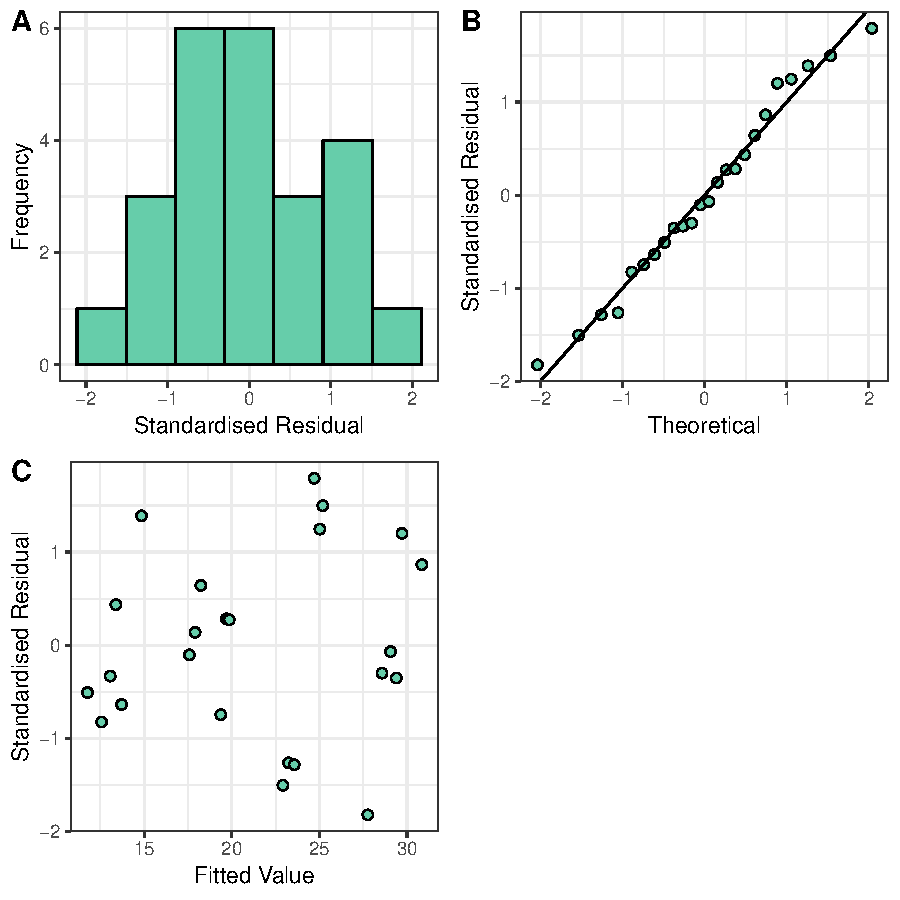
\includegraphics[width=0.5\textwidth]{GoodResplot.pdf}
\end{frame}

%%%%%%%%%%%%%%%%%%%%%%%%%%%%%%%%%%%%%%%%%%%%%%%%%%%%%%%%%%%%%%%%%%%%%%%%%%%%%%%%%%%%%%%%%%%%%%%%%%%
% Slide
%%%%%%%%%%%%%%%%%%%%%%%%%%%%%%%%%%%%%%%%%%%%%%%%%%%%%%%%%%%%%%%%%%%%%%%%%%%%%%%%%%%%%%%%%%%%%%%%%%%
\begin{frame}\frametitle{Model Assumptions}
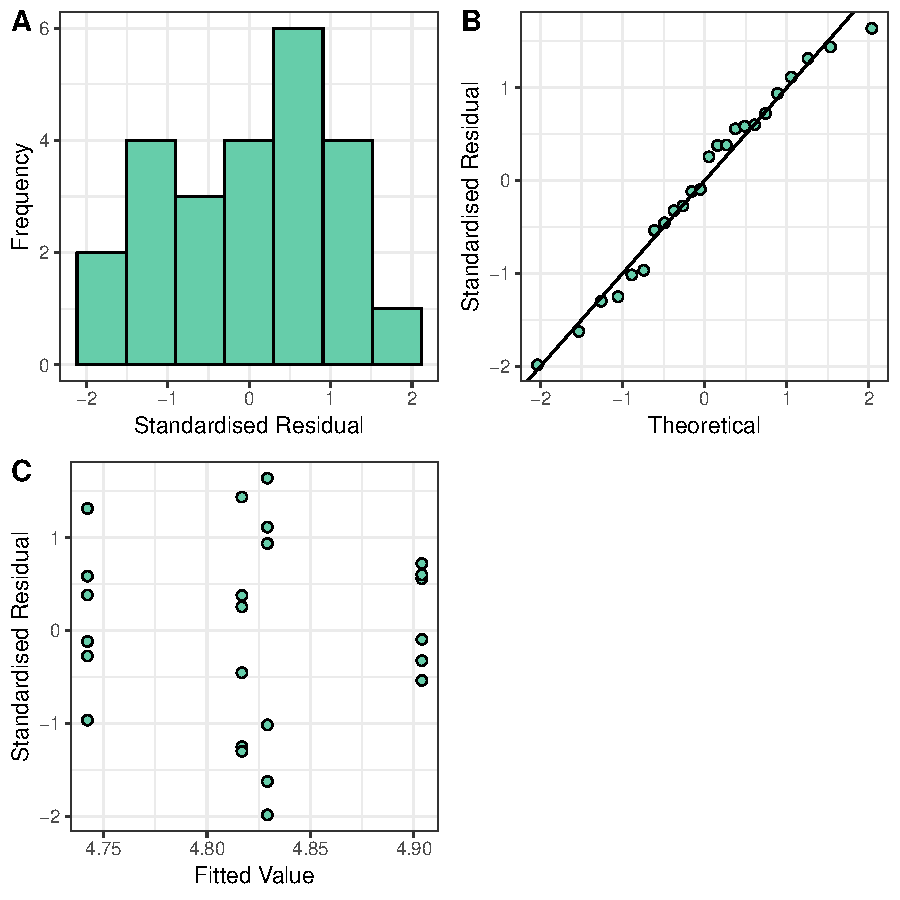
\includegraphics[width=0.5\textwidth]{OKResplot.pdf}
\end{frame}

%%%%%%%%%%%%%%%%%%%%%%%%%%%%%%%%%%%%%%%%%%%%%%%%%%%%%%%%%%%%%%%%%%%%%%%%%%%%%%%%%%%%%%%%%%%%%%%%%%%
% Slide
%%%%%%%%%%%%%%%%%%%%%%%%%%%%%%%%%%%%%%%%%%%%%%%%%%%%%%%%%%%%%%%%%%%%%%%%%%%%%%%%%%%%%%%%%%%%%%%%%%%
\begin{frame}\frametitle{Model Assumptions}
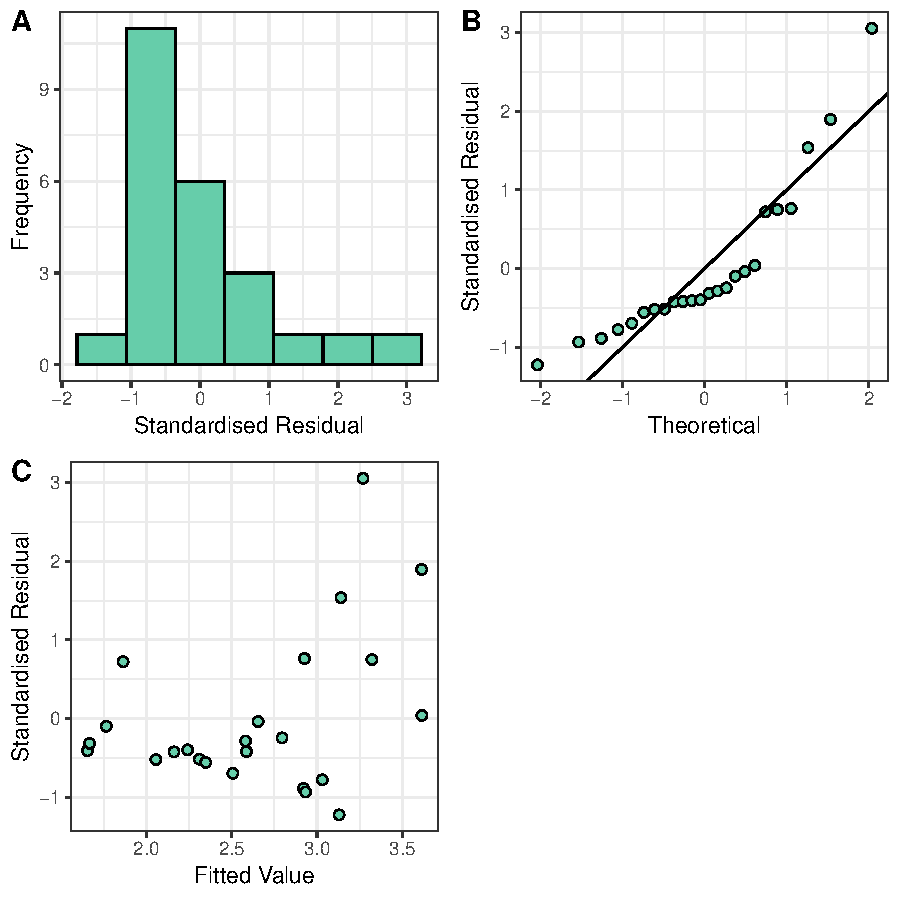
\includegraphics[width=0.5\textwidth]{BadResplot.pdf}
\end{frame}

%%%%%%%%%%%%%%%%%%%%%%%%%%%%%%%%%%%%%%%%%%%%%%%%%%%%%%%%%%%%%%%%%%%%%%%%%%%%%%%%%%%%%%%%%%%%%%%%%%%
% Slide
%%%%%%%%%%%%%%%%%%%%%%%%%%%%%%%%%%%%%%%%%%%%%%%%%%%%%%%%%%%%%%%%%%%%%%%%%%%%%%%%%%%%%%%%%%%%%%%%%%%
\begin{frame}\frametitle{Model Assumptions - heterogeneity}
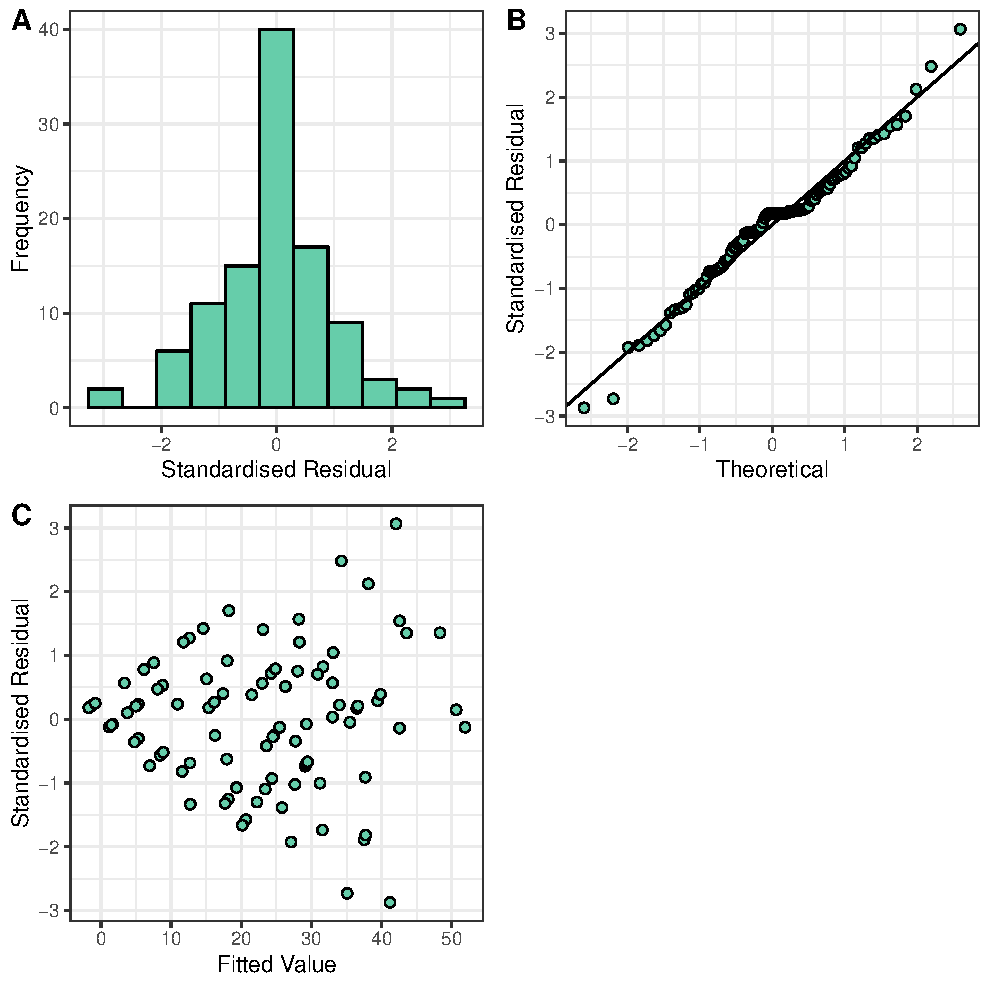
\includegraphics[width=0.5\textwidth]{HeterogenietyResplot.pdf}
\end{frame}



%%%%%%%%%%%%%%%%%%%%%%%%%%%%%%%%%%%%%%%%%%%%%%%%%%%%%%%%%%%%%%%%%%%%%%%%%%%%%%%%%%%%%%%%%%%%%%%%%%%
% Slide
%%%%%%%%%%%%%%%%%%%%%%%%%%%%%%%%%%%%%%%%%%%%%%%%%%%%%%%%%%%%%%%%%%%%%%%%%%%%%%%%%%%%%%%%%%%%%%%%%%%
\begin{frame}\frametitle{Fitting the Model}
Fitting the model is simply the physical process of running the model to analyse the data in a statistical package. In
this case we use the R statistical package \cite{r}. There are a number of different functions in R and other packages
that will allow the analysis of this experiment - for this analysis we will use the standard function \texttt{aov}.

\vspace{3cm}
\flushright

\includegraphics[height = 0.3cm]{yourturn}

\end{frame}



%%%%%%%%%%%%%%%%%%%%%%%%%%%%%%%%%%%%%%%%%%%%%%%%%%%%%%%%%%%%%%%%%%%%%%%%%%%%%%%%%%%%%%%%%%%%%%%%%%%
% Slide
%%%%%%%%%%%%%%%%%%%%%%%%%%%%%%%%%%%%%%%%%%%%%%%%%%%%%%%%%%%%%%%%%%%%%%%%%%%%%%%%%%%%%%%%%%%%%%%%%%%
\begin{frame}\frametitle{Interpreting the Output}
The model assumptions need to be verified before the statistical inferences can be considered. Assumption 4 is assessed
using the first two graphs in the output (A and B) - the histogram and the QQ-plot. The histogram of the residuals
should be approximately symmetrical and bell-shaped, centred around zero. The QQ-plot displays the ordered residuals
plotted against the quantiles of the (in this case) Normal distribution. Deviations from the straight line indicates
deviation from the Normal distribution.

\end{frame}



%%%%%%%%%%%%%%%%%%%%%%%%%%%%%%%%%%%%%%%%%%%%%%%%%%%%%%%%%%%%%%%%%%%%%%%%%%%%%%%%%%%%%%%%%%%%%%%%%%%
% Slide
%%%%%%%%%%%%%%%%%%%%%%%%%%%%%%%%%%%%%%%%%%%%%%%%%%%%%%%%%%%%%%%%%%%%%%%%%%%%%%%%%%%%%%%%%%%%%%%%%%%
\begin{frame}\frametitle{The Shapiro-Wilk test of normality}
\begin{align*}
& H_0: \texttt{The data are normally distributed}\\
& H_1: \texttt{The data are not normally distributed}\\
\end{align*}
and for the assumption the residuals are normally distributed to be met, the p-value associated with the Shapiro-Wilk's
test needs to be $\ge$ 0.05.

\end{frame}



%%%%%%%%%%%%%%%%%%%%%%%%%%%%%%%%%%%%%%%%%%%%%%%%%%%%%%%%%%%%%%%%%%%%%%%%%%%%%%%%%%%%%%%%%%%%%%%%%%%
% Slide
%%%%%%%%%%%%%%%%%%%%%%%%%%%%%%%%%%%%%%%%%%%%%%%%%%%%%%%%%%%%%%%%%%%%%%%%%%%%%%%%%%%%%%%%%%%%%%%%%%%
\begin{frame}\frametitle{Scientific Notation}
Note: statistical packages display numbers in scientific notation as \texttt{9.41e-10}. This number is written in
scientific notation as $9.41\times 10^{-10}$.

\vspace{2cm}
\centering
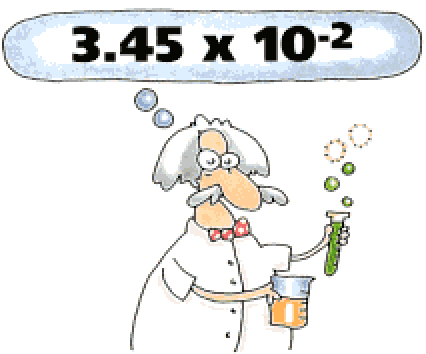
\includegraphics[height = 3cm]{scinot}

\end{frame}



%%%%%%%%%%%%%%%%%%%%%%%%%%%%%%%%%%%%%%%%%%%%%%%%%%%%%%%%%%%%%%%%%%%%%%%%%%%%%%%%%%%%%%%%%%%%%%%%%%%
% Slide
%%%%%%%%%%%%%%%%%%%%%%%%%%%%%%%%%%%%%%%%%%%%%%%%%%%%%%%%%%%%%%%%%%%%%%%%%%%%%%%%%%%%%%%%%%%%%%%%%%%
\begin{frame}\frametitle{Example 1 - Prediction}
The analysis of variance provides estimates for each treatment mean. These estimated
treatment means are the predicted values of the model.


\vspace{2cm}
\centering
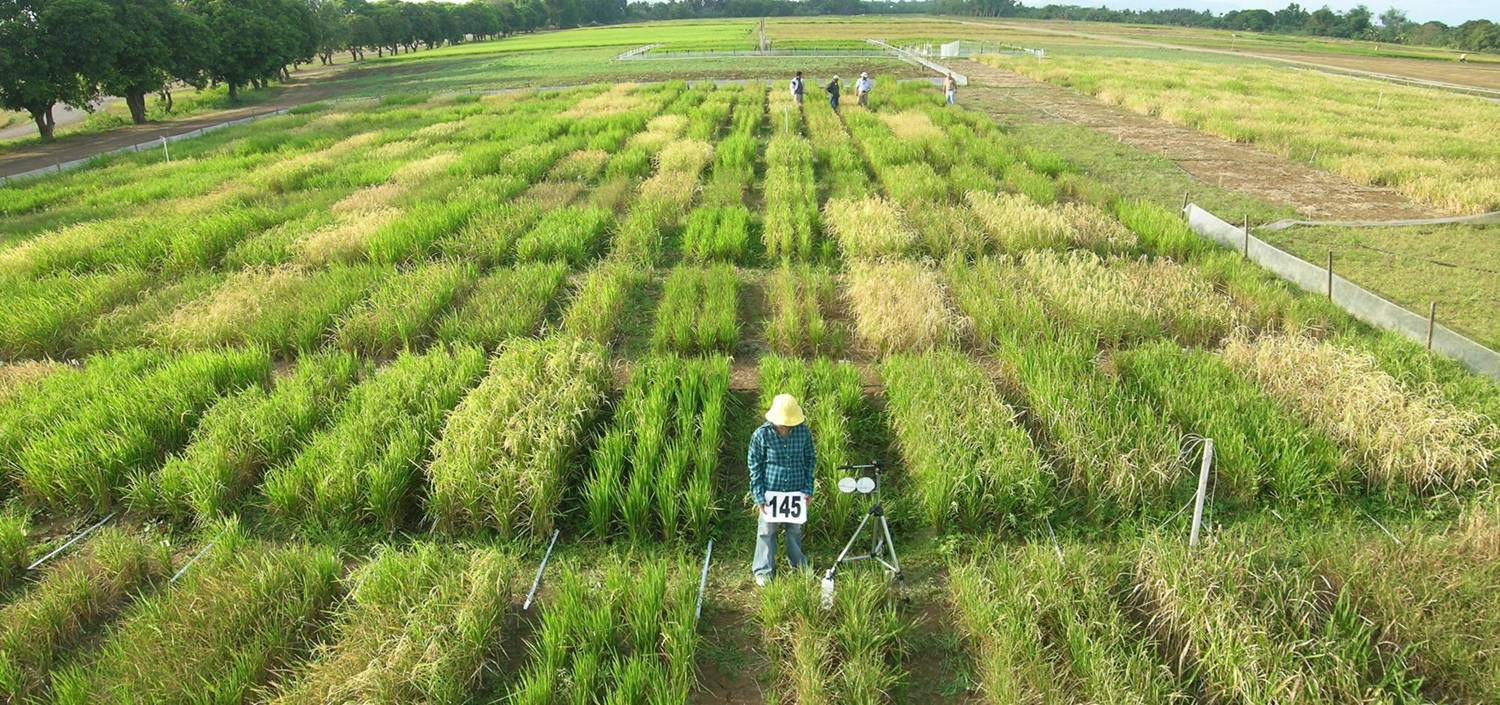
\includegraphics[height = 5cm]{crdwheat}
\vspace{0.1cm}
\flushright

\includegraphics[height = 0.3cm]{yourturn}

\end{frame}




%%%%%%%%%%%%%%%%%%%%%%%%%%%%%%%%%%%%%%%%%%%%%%%%%%%%%%%%%%%%%%%%%%%%%%%%%%%%%%%%%%%%%%%%%%%%%%%%%%%
% Slide
%%%%%%%%%%%%%%%%%%%%%%%%%%%%%%%%%%%%%%%%%%%%%%%%%%%%%%%%%%%%%%%%%%%%%%%%%%%%%%%%%%%%%%%%%%%%%%%%%%%

\begin{frame}\frametitle{Looking at the predicted values}
Calcium concentration 10 has the highest predicted value of
17.8cm ($\pm$0.40cm) and Calcium concentration 20 has the
lowest predicted value of 10.0cm ($\pm$0.40cm).
\end{frame}


%%%%%%%%%%%%%%%%%%%%%%%%%%%%%%%%%%%%%%%%%%%%%%%%%%%%%%%%%%%%%%%%%%%%%%%%%%%%%%%%%%%%%%%%%%%%%%%%%%%
% Slide
%%%%%%%%%%%%%%%%%%%%%%%%%%%%%%%%%%%%%%%%%%%%%%%%%%%%%%%%%%%%%%%%%%%%%%%%%%%%%%%%%%%%%%%%%%%%%%%%%%%
\begin{frame}\frametitle{Multiple Comparison Test}
The aim of this analysis was to determine the effect of the treatments. We have found a significant effect of treatment
on root length. When you want to determine the treatment differences you need to compare each treatment to every other
treatment. In the case where there are 4 treatments (as in Example 1), there are a total of 6 comparisons that need to
be made, to compare each treatment with all the other treatments - for more treatments many more comparisons are
required. In this situation it has been shown that the Type I error can be seriously compromised and the Type I error
for all the comparisons can end up being larger than expected. To adjust for this a \textbf{family-wise} Type I error
rate is employed and the method of comparison is called Tukey's Multiple Comparison Test.


\vspace{1cm}
\flushright

\includegraphics[height = 0.3cm]{yourturn}

\end{frame}


%%%%%%%%%%%%%%%%%%%%%%%%%%%%%%%%%%%%%%%%%%%%%%%%%%%%%%%%%%%%%%%%%%%%%%%%%%%%%%%%%%%%%%%%%%%%%%%%%%%
% Slide
%%%%%%%%%%%%%%%%%%%%%%%%%%%%%%%%%%%%%%%%%%%%%%%%%%%%%%%%%%%%%%%%%%%%%%%%%%%%%%%%%%%%%%%%%%%%%%%%%%%

\begin{frame}\frametitle{Looking at the multiple comparison test}
At the family 5\% significance level:
\begin{itemize}
\item The two middle concentrations are not significantly different
\item Calcium concentration 1 is significantly higher than concentration
             20 but significantly lower than concentrations 5 and 10.
\item Calcium concentration 20 is significantly lower than all other concentrations
\end{itemize}
\end{frame}




%%%%%%%%%%%%%%%%%%%%%%%%%%%%%%%%%%%%%%%%%%%%%%%%%%%%%%%%%%%%%%%%%%%%%%%%%%%%%%%%%%%%%%%%%%%%%%%%%%%
% Slide
%%%%%%%%%%%%%%%%%%%%%%%%%%%%%%%%%%%%%%%%%%%%%%%%%%%%%%%%%%%%%%%%%%%%%%%%%%%%%%%%%%%%%%%%%%%%%%%%%%%
\begin{frame}\frametitle{Example 2}
An experiment was run to investigate the effect of the differences in seven treatments in reducing scab disease in
potatoes. The experimental material consisted of 84 field plots arranged in a rectangular array of six rows and 14
columns. Each treatment was applied to 12 plots selected at random to give a CRD design. The response is the average
tuber length growth over a seven day period. The data can be found in \texttt{example2.csv}.


The analysis will be undertaken to determine
\begin{eqnarray*}
	H_0&:& \mu_{T1} = \mu_{T2} = \hdots = \mu_{T7} \\
	H_1&:& \texttt{not all the treatment means are the same}
\end{eqnarray*}
\end{frame}


%%%%%%%%%%%%%%%%%%%%%%%%%%%%%%%%%%%%%%%%%%%%%%%%%%%%%%%%%%%%%%%%%%%%%%%%%%%%%%%%%%%%%%%%%%%%%%%%%%%
% Slide
%%%%%%%%%%%%%%%%%%%%%%%%%%%%%%%%%%%%%%%%%%%%%%%%%%%%%%%%%%%%%%%%%%%%%%%%%%%%%%%%%%%%%%%%%%%%%%%%%%%
\begin{frame}\frametitle{Experimental Layout}

\begin{center}
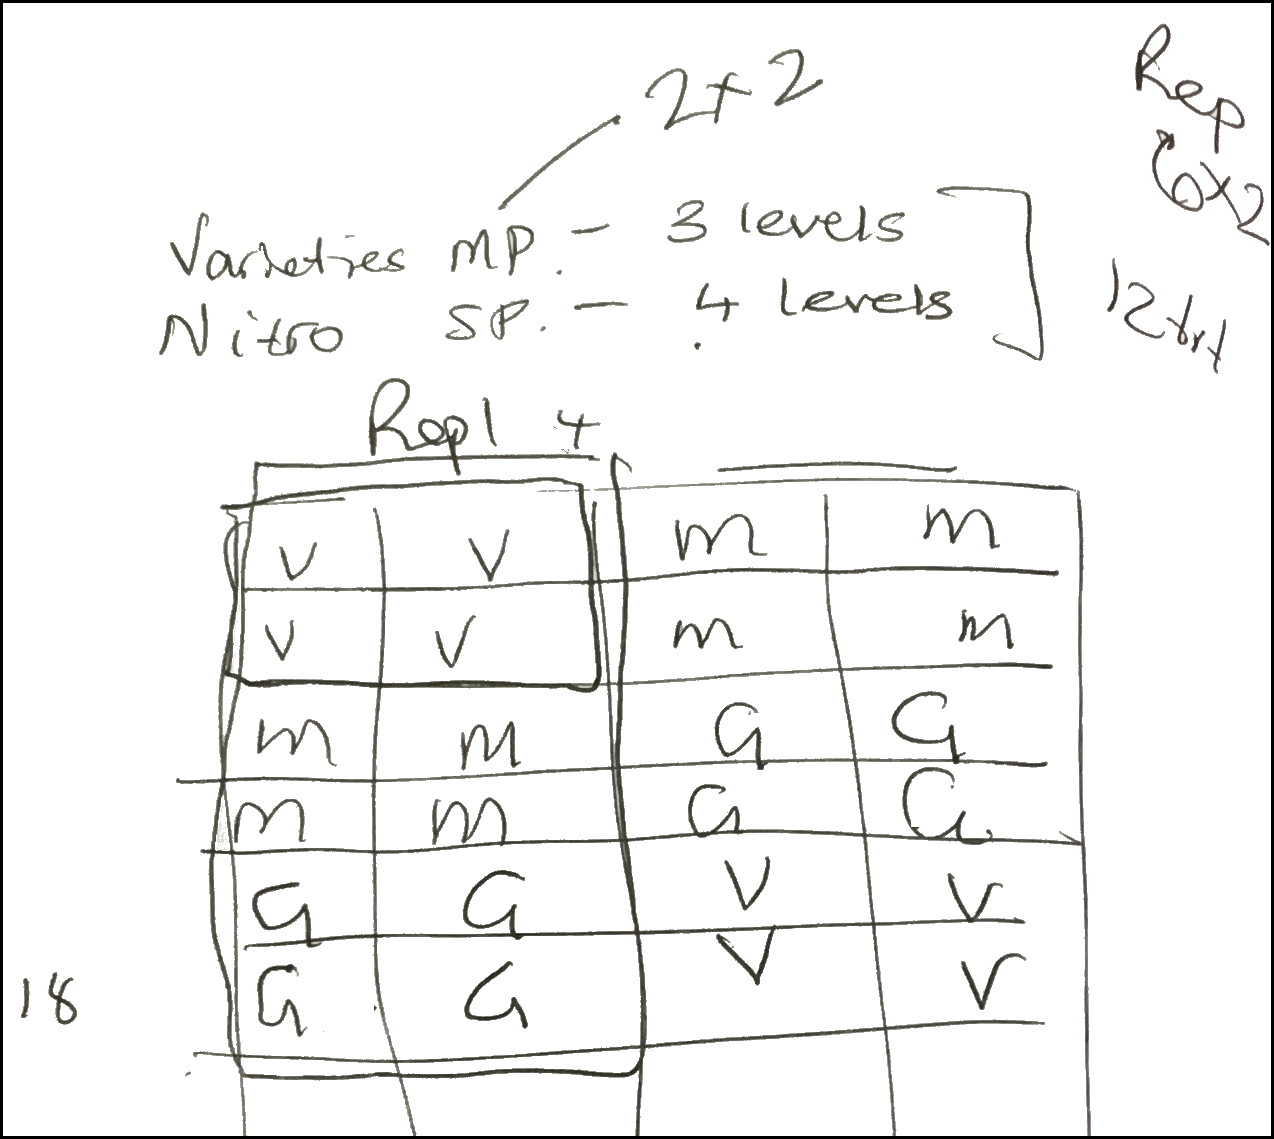
\includegraphics[height = 0.7\textheight]{exptlayout.png}
\end{center}
\flushright

\includegraphics[height = 0.3cm]{yourturn}
\end{frame}


%%%%%%%%%%%%%%%%%%%%%%%%%%%%%%%%%%%%%%%%%%%%%%%%%%%%%%%%%%%%%%%%%%%%%%%%%%%%%%%%%%%%%%%%%%%%%%%%%%%
% Slide
%%%%%%%%%%%%%%%%%%%%%%%%%%%%%%%%%%%%%%%%%%%%%%%%%%%%%%%%%%%%%%%%%%%%%%%%%%%%%%%%%%%%%%%%%%%%%%%%%%%

\begin{frame}\frametitle{Looking at the predicted values}
Treatment T3 has the lowest predicted value of 11.2mm ($\pm$0.33mm)
and T1 has the highest predicted value of 17.8mm
($\pm$0.33cm).
\end{frame}

%%%%%%%%%%%%%%%%%%%%%%%%%%%%%%%%%%%%%%%%%%%%%%%%%%%%%%%%%%%%%%%%%%%%%%%%%%%%%%%%%%%%%%%%%%%%%%%%%%%
% Slide
%%%%%%%%%%%%%%%%%%%%%%%%%%%%%%%%%%%%%%%%%%%%%%%%%%%%%%%%%%%%%%%%%%%%%%%%%%%%%%%%%%%%%%%%%%%%%%%%%%%

\begin{frame}\frametitle{Looking at the multiple comparison test}
At the family 5\% significance level:
\begin{itemize}
\item T1 and T7 are not significantly different but T1 is significantly higher than
the other treatments
\item T2 is not significantly different from T4 or T7
\item T3 is not significantly different T5
\item T4 is not significantly different T2 or T6
\item T6 is not significantly different T4
\item T7 is not significantly different from T1 or T2
\end{itemize}
\end{frame}


%%%%%%%%%%%%%%%%%%%%%%%%%%%%%%%%%%%%%%%%%%%%%%%%%%%%%%%%%%%%%%%%%%%%%%%%%%%%%%%%%%%%%%%%%%%%%%%%%%%
% Slide
%%%%%%%%%%%%%%%%%%%%%%%%%%%%%%%%%%%%%%%%%%%%%%%%%%%%%%%%%%%%%%%%%%%%%%%%%%%%%%%%%%%%%%%%%%%%%%%%%%%

\begin{frame}[fragile]\frametitle{Exercise 1}
\begin{verbatim}
Response: Yield
          Df  Sum Sq  Mean Sq F value    Pr(>F)
Variety   11 2.14254 0.194777  4.6796 0.0007707 ***
Residuals 24 0.99893 0.041622

            Yield groups
Arrino   2.753333      a
Pugsley  2.750000      a
Caryina  2.540000     ab
Fortune  2.526667     ab
Zippy    2.283333     ab
Orion    2.270000     ab
Endure   2.240000     ab
Janz     2.193333     ab
Baxter   2.140000      b
Drysdale 2.130000      b
Wylah    2.130000      b
Lang     1.973333      b
\end{verbatim}
\end{frame}




\begin{frame}[fragile]\frametitle{Exercise 2}
\begin{verbatim}
Response: Time
          Df Sum Sq Mean Sq F value   Pr(>F)
Treatment  5 4.2352 0.84704  6.4554 0.001331 **
Residuals 18 2.3619 0.13122


     Time groups
CP 3.3650      a
HE 2.7975     ab
CN 2.7700     ab
HL 2.6150     ab
PE 2.1650      b
KC 2.1250      b
\end{verbatim}
\end{frame}

\subsection{Randomised Complete Block Design}
%%%%%%%%%%%%%%%%%%%%%%%%%%%%%%%%%%%%%%%%%%%%%%%%%%%%%%%%%%%%%%%%%%%%%%%%%%%%%%%%%%%%%%%%%%%%%%%%%%%
% Slide
%%%%%%%%%%%%%%%%%%%%%%%%%%%%%%%%%%%%%%%%%%%%%%%%%%%%%%%%%%%%%%%%%%%%%%%%%%%%%%%%%%%%%%%%%%%%%%%%%%%
\begin{frame}[fragile]\frametitle{Randomised Complete Block Design (RCBD)}
The simplest design that includes blocking and is probably the most
frequently used design in research. In this design the number of experimental units in each block must equal the number
of treatments. Within each block, treatments are then randomly allocated within each block. As the design is carried
out taking into account the blocks, these are also fitted in the model when analysing the data.

\begin{verbatim}
Source of Variation                      df
===================================================
Block stratum                            b-1
---------------------------------------------------
trt                                      t-1
Residual                                 (b-1)(t-1)
===================================================
Total                                    bt-1
\end{verbatim}

where $t$ are the number of treatments and $b$ is the number of blocks.

\end{frame}


%%%%%%%%%%%%%%%%%%%%%%%%%%%%%%%%%%%%%%%%%%%%%%%%%%%%%%%%%%%%%%%%%%%%%%%%%%%%%%%%%%%%%%%%%%%%%%%%%%%
% Slide
%%%%%%%%%%%%%%%%%%%%%%%%%%%%%%%%%%%%%%%%%%%%%%%%%%%%%%%%%%%%%%%%%%%%%%%%%%%%%%%%%%%%%%%%%%%%%%%%%%%
\begin{frame}\frametitle{RCBD - variance partitioning}
\centering
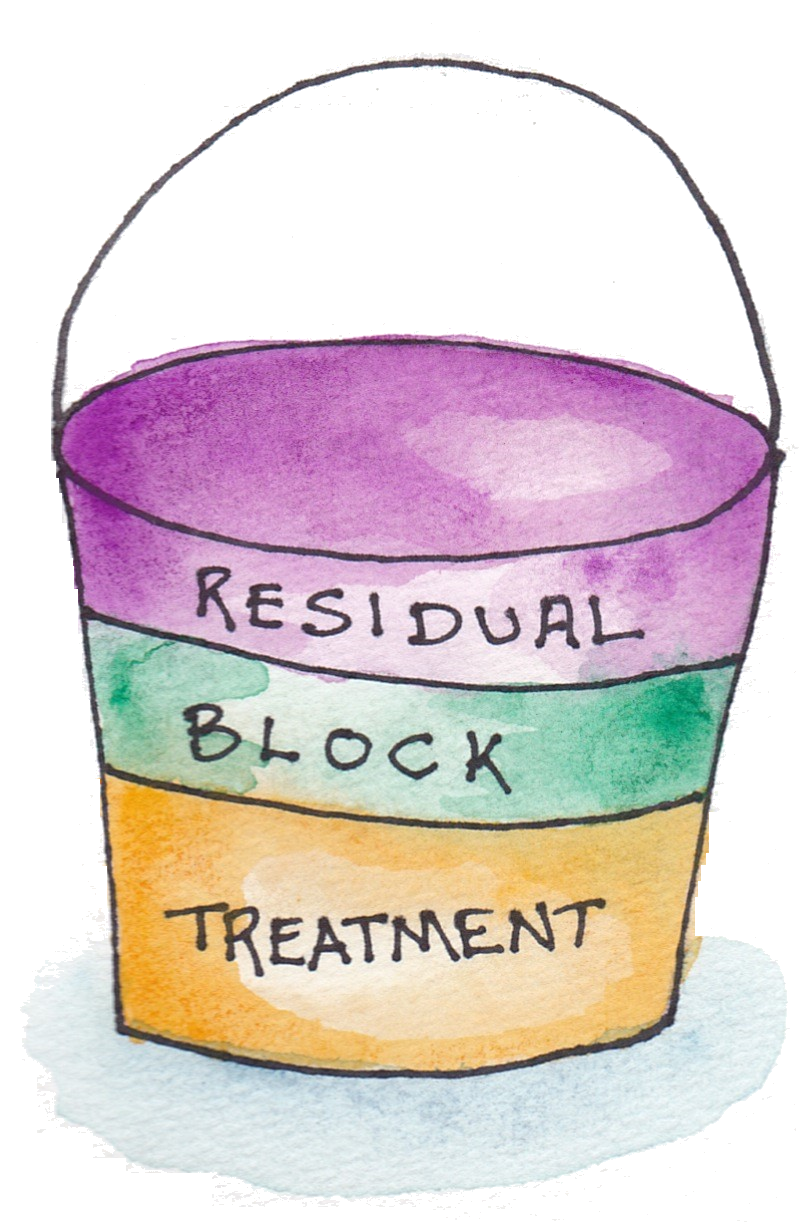
\includegraphics[width = 4cm]{rcbdbucket.png}
\end{frame}



%%%%%%%%%%%%%%%%%%%%%%%%%%%%%%%%%%%%%%%%%%%%%%%%%%%%%%%%%%%%%%%%%%%%%%%%%%%%%%%%%%%%%%%%%%%%%%%%%%%
% Slide
%%%%%%%%%%%%%%%%%%%%%%%%%%%%%%%%%%%%%%%%%%%%%%%%%%%%%%%%%%%%%%%%%%%%%%%%%%%%%%%%%%%%%%%%%%%%%%%%%%%
\begin{frame}\frametitle{RCBD ANOVA Table}
\footnotesize
\begin{tabular}{llllc}
\hline
   & & & &\\
  Source & SS & df & MS & F \\
   & & & &\\
  Treatment & $b \sum_{i=1}^{t} (\bar{y}_{i}-\bar{y})^2$ & $t-1$ & $\frac{SS_{Trt}}{t-1}$ & $\frac{MS_{Trt}}{MS_{Residual}}$ \\
   & & & &\\
  Block & $t \sum_{j=1}^{b} (\bar{y}_{j}-\bar{y})^2$ & $b-1$ & $\frac{SS_{Block}}{b-1}$ & \\
   & & & &\\
  Residual & $\sum_{i=1}^{t} \sum_{j=1}^{b} (\bar{y}_{ij}-\bar{y}_{i}-\bar{y}_{j} + \bar{y})^2$ & $(t-1)(b-1)$ & $\frac{SS_{Residual}}{(t-1)(b-1)}$ &  \\
   & & & &\\
   Total & $\sum_{i=1}^{t} \sum_{j=1}^{b} (\bar{y}_{ij}-\bar{y})^2 $ & $tb-1$ &  &  \\
   & & & &\\
  \hline
\end{tabular} \\

\end{frame}


%%%%%%%%%%%%%%%%%%%%%%%%%%%%%%%%%%%%%%%%%%%%%%%%%%%%%%%%%%%%%%%%%%%%%%%%%%%%%%%%%%%%%%%%%%%%%%%%%%%
% Slide
%%%%%%%%%%%%%%%%%%%%%%%%%%%%%%%%%%%%%%%%%%%%%%%%%%%%%%%%%%%%%%%%%%%%%%%%%%%%%%%%%%%%%%%%%%%%%%%%%%%
\begin{frame}\frametitle{RCBD Hypotheses}
The main hypothesis of interest when analysing a randomised complete block design is the test for treatment effects.

\begin{eqnarray*}
H_0:& \texttt{all } \alpha_i = 0 \\
H_1:& \texttt{not all } \alpha_i \texttt{ are equal to zero} \\
\end{eqnarray*}\

or equivalently the test to determine whether the treatment means differ.

\begin{eqnarray*}
H_0:& \texttt{all } \mu_i \texttt{ are the same} \\
H_1:& \texttt{not all } \mu_i \texttt{ are the same} \\
\end{eqnarray*}
\end{frame}





%%%%%%%%%%%%%%%%%%%%%%%%%%%%%%%%%%%%%%%%%%%%%%%%%%%%%%%%%%%%%%%%%%%%%%%%%%%%%%%%%%%%%%%%%%%%%%%%%%%
% Slide
%%%%%%%%%%%%%%%%%%%%%%%%%%%%%%%%%%%%%%%%%%%%%%%%%%%%%%%%%%%%%%%%%%%%%%%%%%%%%%%%%%%%%%%%%%%%%%%%%%%
\begin{frame}\frametitle{Example 3}

A researcher wants to test for varietal differences between 4 varieties of field peas. Based on the information gained
during previous trials it was known that 5 replicates are required. The researcher used a randomised complete block
design, as there were known field trends that make using a randomised complete block a sensible option. The data can be
found in  \texttt{example3.csv}.

\vspace{1cm}
\centering
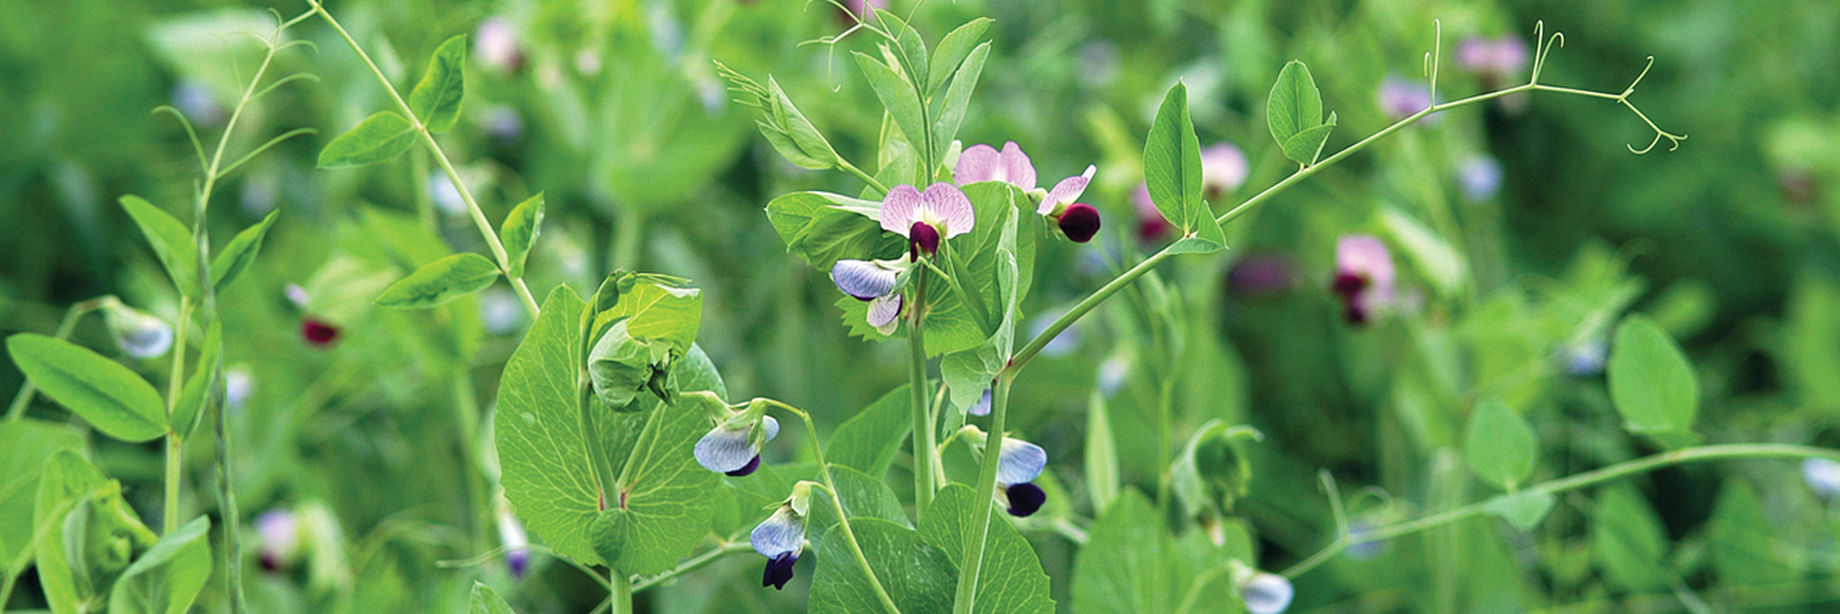
\includegraphics[width = 8cm]{fpeas}

\end{frame}


%%%%%%%%%%%%%%%%%%%%%%%%%%%%%%%%%%%%%%%%%%%%%%%%%%%%%%%%%%%%%%%%%%%%%%%%%%%%%%%%%%%%%%%%%%%%%%%%%%%
% Slide
%%%%%%%%%%%%%%%%%%%%%%%%%%%%%%%%%%%%%%%%%%%%%%%%%%%%%%%%%%%%%%%%%%%%%%%%%%%%%%%%%%%%%%%%%%%%%%%%%%%
\begin{frame}\frametitle{Example 3}
\footnotesize
\begin{center}
\begin{tabular}{|c|c|c|c|c|c|}
  \hline
   & Col 1 & Col 2 & Col 3 & Col 4 & Col 5 \\
  \hline
  Row 1 & Parafield (0.45) & Yarrum (2.95) & Excell (6.28) & Kaspa (3.29) & Yarrum (8.20) \\
  \hline
  Row 2 & Yarrum (5.28) & Parafield (1.70) & Kaspa (0.30) & Yarrum (3.45) & Excell (5.14) \\
  \hline
  Row 3 & Excell (2.94) & Kaspa (1.94) & Parafield (1.69) & Parafield (0.04) & Kaspa (5.68) \\
  \hline
  Row 4 & Kaspa (2.17) & Excell (5.56) & Yarrum (3.74) & Excell (4.32) & Parafield (4.52) \\
  \hline
\end{tabular} \\
\end{center}

\end{frame}


%%%%%%%%%%%%%%%%%%%%%%%%%%%%%%%%%%%%%%%%%%%%%%%%%%%%%%%%%%%%%%%%%%%%%%%%%%%%%%%%%%%%%%%%%%%%%%%%%%%
% Slide
%%%%%%%%%%%%%%%%%%%%%%%%%%%%%%%%%%%%%%%%%%%%%%%%%%%%%%%%%%%%%%%%%%%%%%%%%%%%%%%%%%%%%%%%%%%%%%%%%%%
\begin{frame}\frametitle{Experimental Layout}

\begin{center}
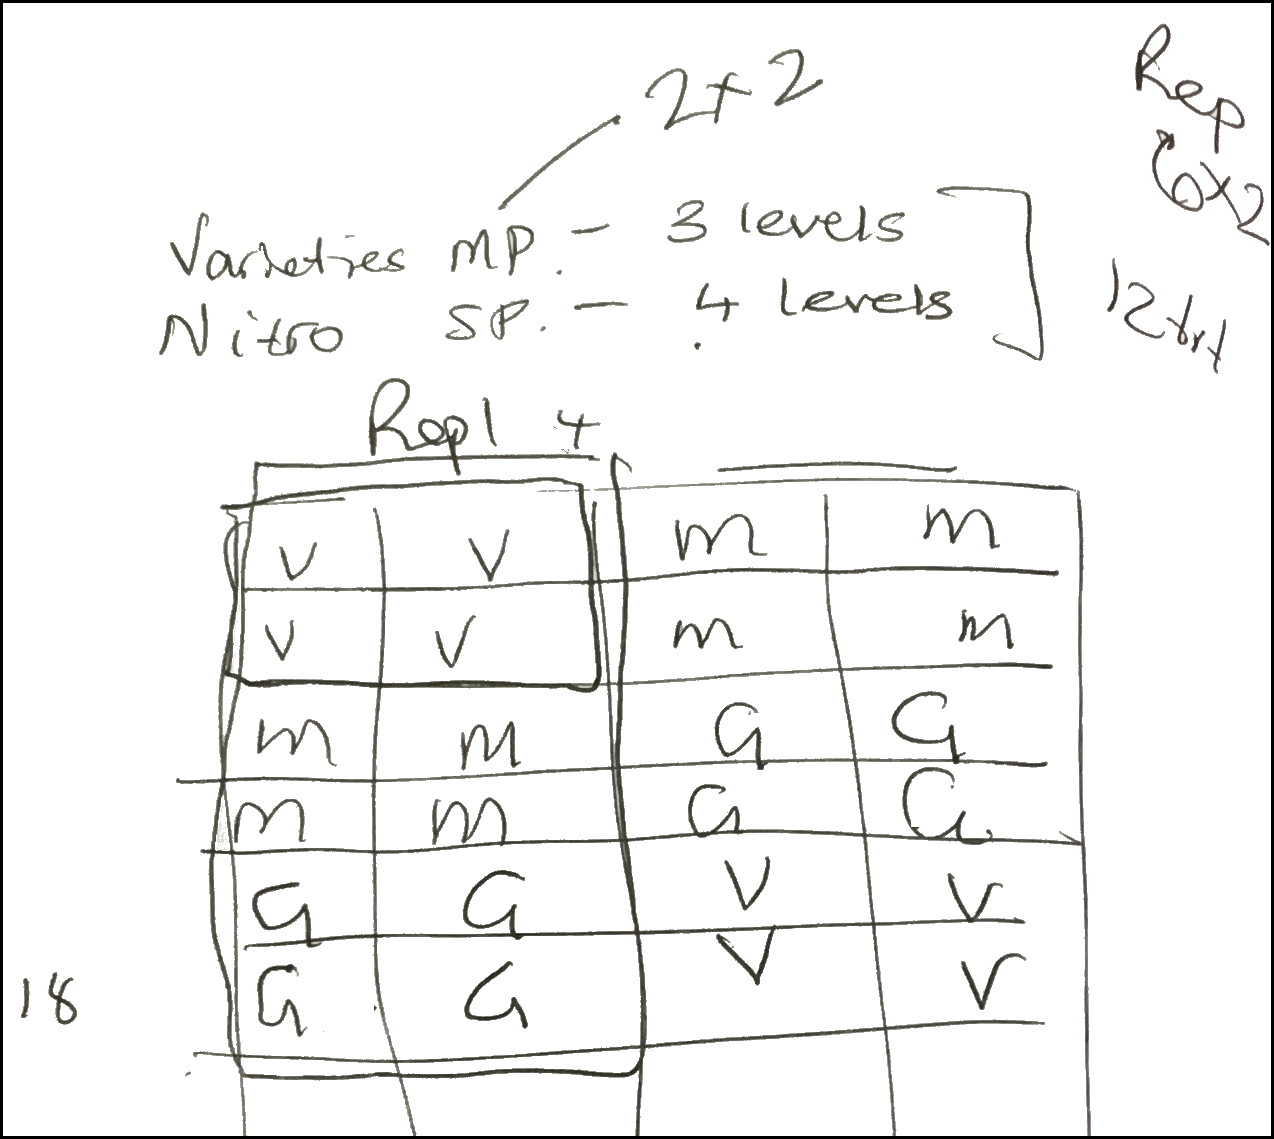
\includegraphics[height = 0.7\textheight]{exptlayout.png}
\end{center}
\flushright

\includegraphics[height = 0.3cm]{yourturn}
\end{frame}


%%%%%%%%%%%%%%%%%%%%%%%%%%%%%%%%%%%%%%%%%%%%%%%%%%%%%%%%%%%%%%%%%%%%%%%%%%%%%%%%%%%%%%%%%%%%%%%%%%%
% Slide
%%%%%%%%%%%%%%%%%%%%%%%%%%%%%%%%%%%%%%%%%%%%%%%%%%%%%%%%%%%%%%%%%%%%%%%%%%%%%%%%%%%%%%%%%%%%%%%%%%%
\begin{frame}\frametitle{Example 3}
\begin{enumerate}
\item The null hypothesis is that all the varieties will have the same yield, that is:
\begin{align*}
& H_0: \texttt{The fieldpea yield is not dependent on the variety}\\
& H_1:\texttt{The fieldpea yield is dependent on the variety}\\
\end{align*}
\item A randomised complete block design has been used. \\
\item The treatments are the varieties.\\
\item The experimental unit is the plot, as the varieties have been randomised to the plots.\\
\item The observational unit is also the plot, as the whole plot was harvested to give the yield measurement.\\
\item The experiment was conducted in the field in a rectangular array of rows and columns.\\
\end{enumerate}

\end{frame}


%%%%%%%%%%%%%%%%%%%%%%%%%%%%%%%%%%%%%%%%%%%%%%%%%%%%%%%%%%%%%%%%%%%%%%%%%%%%%%%%%%%%%%%%%%%%%%%%%%%
% Slide
%%%%%%%%%%%%%%%%%%%%%%%%%%%%%%%%%%%%%%%%%%%%%%%%%%%%%%%%%%%%%%%%%%%%%%%%%%%%%%%%%%%%%%%%%%%%%%%%%%%
\begin{frame}\frametitle{RCBD - Linear Model}
The linear model that is fit can be symbolically written as:
\begin{eqnarray*}
	\texttt{Response variable}&:& \texttt{Yield} \\
	\texttt{Structural component}&:& \texttt{Block}\\
	\texttt{Explanatory component}&:& \texttt{Variety}\\
	\texttt{Residual}&:& \texttt{Assume Independence}
\end{eqnarray*}
\end{frame}




%%%%%%%%%%%%%%%%%%%%%%%%%%%%%%%%%%%%%%%%%%%%%%%%%%%%%%%%%%%%%%%%%%%%%%%%%%%%%%%%%%%%%%%%%%%%%%%%%%%
% Slide
%%%%%%%%%%%%%%%%%%%%%%%%%%%%%%%%%%%%%%%%%%%%%%%%%%%%%%%%%%%%%%%%%%%%%%%%%%%%%%%%%%%%%%%%%%%%%%%%%%%
\begin{frame}\frametitle{Example 4}
\begin{enumerate}
\item The null hypothesis is that all the soil types will have the same Dry Matter, that is:
\begin{align*}
& H_0: \texttt{The lupin dry matter is not dependent on the soil type}\\
& H_1:\texttt{The lupin dry matter is dependent on the soil type}\\
\end{align*}
\item A Latin square design has been used. \\
\item The treatments are the soil types.\\
\item The experimental unit is the pot, as the soil types have been randomised to the pots.\\
\item The observational unit is also the pot.\\
\item The experiment was conducted in the glasshouse in a rectangular array of rows and columns.\\
\end{enumerate}
\end{frame}

%%%%%%%%%%%%%%%%%%%%%%%%%%%%%%%%%%%%%%%%%%%%%%%%%%%%%%%%%%%%%%%%%%%%%%%%%%%%%%%%%%%%%%%%%%%%%%%%%%%
% Slide
%%%%%%%%%%%%%%%%%%%%%%%%%%%%%%%%%%%%%%%%%%%%%%%%%%%%%%%%%%%%%%%%%%%%%%%%%%%%%%%%%%%%%%%%%%%%%%%%%%%

\begin{frame}\frametitle{Looking at the multiple comparison test}
At the family 5\% significance level:
\begin{itemize}
\item Excell and Yarrum are not significantly different (to each other)
but both are significantly higher than Parafield
\item Kaspa is not significantly different from any of the other varieties
\item Parafield is significantly lower than Excell and Yarrum
\end{itemize}
\end{frame}


%%%%%%%%%%%%%%%%%%%%%%%%%%%%%%%%%%%%%%%%%%%%%%%%%%%%%%%%%%%%%%%%%%%%%%%%%%%%%%%%%%%%%%%%%%%%%%%%%%%
% Slide
%%%%%%%%%%%%%%%%%%%%%%%%%%%%%%%%%%%%%%%%%%%%%%%%%%%%%%%%%%%%%%%%%%%%%%%%%%%%%%%%%%%%%%%%%%%%%%%%%%%
\begin{frame}[fragile]\frametitle{Exercise 3}
\begin{verbatim}
Response: AverageFruitSize
          Df  Sum Sq Mean Sq F value    Pr(>F)
Replicate  4  44.969 11.2421  12.696 1.092e-05 ***
Variety    6 134.623 22.4371  25.339 2.868e-09 ***
Residuals 24  21.251  0.8855

              AverageFruitSize groups
Sudanese                  8.88      a
Orangeglo                 4.96      b
Melitopolski              4.78      b
Hercules                  4.70     bc
Phantom                   3.08     bc
Pharoah                   2.86      c
CarolinaCross             2.84      c
\end{verbatim}
\end{frame}


%%%%%%%%%%%%%%%%%%%%%%%%%%%%%%%%%%%%%%%%%%%%%%%%%%%%%%%%%%%%%%%%%%%%%%%%%%%%%%%%%%%%%%%%%%%%%%%%%%%
% Slide
%%%%%%%%%%%%%%%%%%%%%%%%%%%%%%%%%%%%%%%%%%%%%%%%%%%%%%%%%%%%%%%%%%%%%%%%%%%%%%%%%%%%%%%%%%%%%%%%%%%
\begin{frame}[fragile]\frametitle{Exercise 4}
\begin{verbatim}
Response: Yield
            Df  Sum Sq Mean Sq F value  Pr(>F)
Block        3 1.94436 0.64812  4.9021 0.01434 *
SeedingRate  5 0.87353 0.17471  1.3214 0.30758
Residuals   15 1.98317 0.13221
\end{verbatim}
\end{frame}

\subsection{Latin Square}
%%%%%%%%%%%%%%%%%%%%%%%%%%%%%%%%%%%%%%%%%%%%%%%%%%%%%%%%%%%%%%%%%%%%%%%%%%%%%%%%%%%%%%%%%%%%%%%%%%%
% Slide
%%%%%%%%%%%%%%%%%%%%%%%%%%%%%%%%%%%%%%%%%%%%%%%%%%%%%%%%%%%%%%%%%%%%%%%%%%%%%%%%%%%%%%%%%%%%%%%%%%%
\begin{frame}\frametitle{Latin Square Design}
The Latin Square Design is where the number of rows and columns has to correspond to the number of treatment levels,
and therefore the number of replicates. The treatment allocation is done so that each treatment occurs once in each
column and row. As the design is carried out taking into account the rows and columns, these are also fitted in the
model when analysing the data.

\vspace{1cm}
\centering
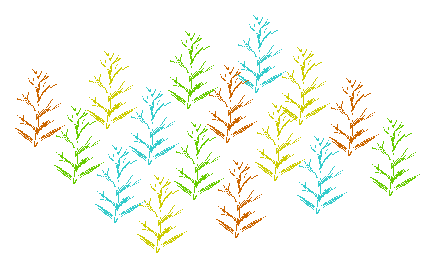
\includegraphics[width = 4cm]{LS}

\end{frame}



%%%%%%%%%%%%%%%%%%%%%%%%%%%%%%%%%%%%%%%%%%%%%%%%%%%%%%%%%%%%%%%%%%%%%%%%%%%%%%%%%%%%%%%%%%%%%%%%%%%
% Slide
%%%%%%%%%%%%%%%%%%%%%%%%%%%%%%%%%%%%%%%%%%%%%%%%%%%%%%%%%%%%%%%%%%%%%%%%%%%%%%%%%%%%%%%%%%%%%%%%%%%
\begin{frame}[fragile]\frametitle{Latin Square ANOVA Table}

\begin{lstlisting}[mathescape=true]
Source of Variation                      df
============================================================
Row                                      (t-1)
Column                                   (t-1)
Treatment                                (t-1)
Residual                                 (t-1)(t-2)
============================================================
Total                                    (t$^2$ - 1)
\end{lstlisting}

where $t$ are the number of treatments.

\end{frame}



%%%%%%%%%%%%%%%%%%%%%%%%%%%%%%%%%%%%%%%%%%%%%%%%%%%%%%%%%%%%%%%%%%%%%%%%%%%%%%%%%%%%%%%%%%%%%%%%%%%
% Slide
%%%%%%%%%%%%%%%%%%%%%%%%%%%%%%%%%%%%%%%%%%%%%%%%%%%%%%%%%%%%%%%%%%%%%%%%%%%%%%%%%%%%%%%%%%%%%%%%%%%
\begin{frame}\frametitle{LSD - Variance Partitioning}
\centering
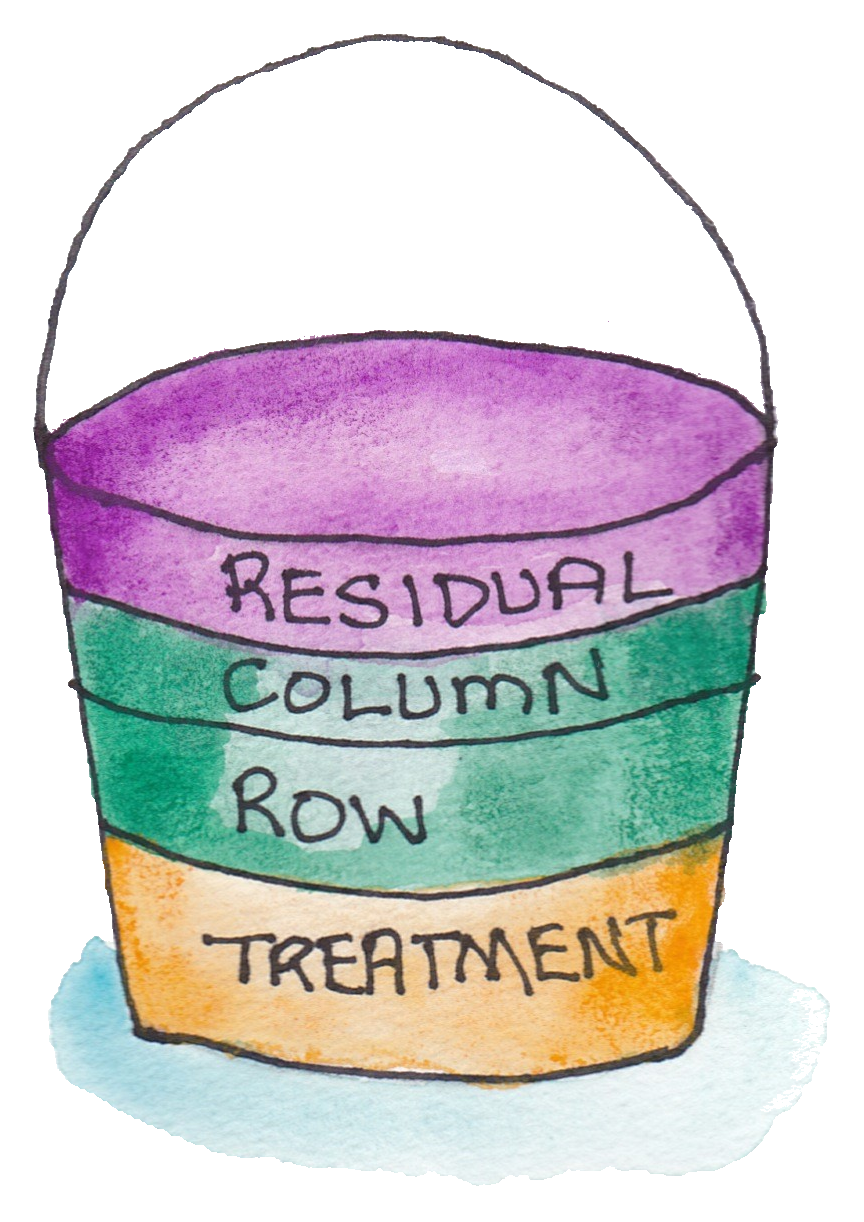
\includegraphics[width = 4cm]{lsbucket.png}

\end{frame}



%%%%%%%%%%%%%%%%%%%%%%%%%%%%%%%%%%%%%%%%%%%%%%%%%%%%%%%%%%%%%%%%%%%%%%%%%%%%%%%%%%%%%%%%%%%%%%%%%%%
% Slide
%%%%%%%%%%%%%%%%%%%%%%%%%%%%%%%%%%%%%%%%%%%%%%%%%%%%%%%%%%%%%%%%%%%%%%%%%%%%%%%%%%%%%%%%%%%%%%%%%%%
\begin{frame}\frametitle{LSD - ANOVA Table}
\footnotesize
\begin{tabular}{llllc}
\hline
   & & & &\\
  Source & SS & df & MS & F \\
   & & & &\\
  Row & $t \sum_{j=1}^{t} (\bar{y}_{j}-\bar{y})^2$ & $t-1$ & $\frac{SS_{Row}}{t-1}$ & \\
   & & & &\\
  Column & $t \sum_{k=1}^{t} (\bar{y}_{k}-\bar{y})^2$ & $t-1$ & $\frac{SS_{Column}}{t-1}$ & \\
   & & & &\\
  Treatment & $t \sum_{i=1}^{t} (\bar{y}_{i}-\bar{y})^2$ & $t-1$ & $\frac{SS_{Trt}}{t-1}$ & $\frac{MS_{Trt}}{MS_{Residual}}$ \\
   & & & &\\
  Residual & $ \sum_{j=1}^{t}\sum_{k=1}^{t} (\bar{y}_{ijk}-\bar{y}_{i}-\bar{y}_{j}-\bar{y}_{k} + 2\bar{y})^2$ & $(t-1)(t-2)$ & $\frac{SS_{Residual}}{(t-1)(t-2)}$ &  \\
   & & & &\\
   Total & $\sum_{i=1}^{t} \sum_{j=1}^{b} (\bar{y}_{ij}-\bar{y})^2 $ & $tb-1$ &  &  \\
   & & & &\\
  \hline
\end{tabular} \\

\end{frame}



%%%%%%%%%%%%%%%%%%%%%%%%%%%%%%%%%%%%%%%%%%%%%%%%%%%%%%%%%%%%%%%%%%%%%%%%%%%%%%%%%%%%%%%%%%%%%%%%%%%
% Slide
%%%%%%%%%%%%%%%%%%%%%%%%%%%%%%%%%%%%%%%%%%%%%%%%%%%%%%%%%%%%%%%%%%%%%%%%%%%%%%%%%%%%%%%%%%%%%%%%%%%
\begin{frame}\frametitle{LSD - hypotheses tests}

The main hypothesis of interest when analysing a Latin square block design is the test for treatment effects.

\begin{eqnarray*}
H_0:& \texttt{all } \alpha_i = 0 \\
H_1:& \texttt{not all } \alpha_i \texttt{ are equal to zero} \\
\end{eqnarray*}\

or equivalently the test to determine whether the treatment means differ.

\begin{eqnarray*}
H_0:& \texttt{all } \mu_i \texttt{ are the same} \\
H_1:& \texttt{not all } \mu_i \texttt{ are the same} \\
\end{eqnarray*}\

\end{frame}



%%%%%%%%%%%%%%%%%%%%%%%%%%%%%%%%%%%%%%%%%%%%%%%%%%%%%%%%%%%%%%%%%%%%%%%%%%%%%%%%%%%%%%%%%%%%%%%%%%%
% Slide
%%%%%%%%%%%%%%%%%%%%%%%%%%%%%%%%%%%%%%%%%%%%%%%%%%%%%%%%%%%%%%%%%%%%%%%%%%%%%%%%%%%%%%%%%%%%%%%%%%%
\begin{frame}\frametitle{Example 4}

An experiment was run to investigate the effects of soil type on the growth of lupins. The experiment was done with
pots on a bench in a glasshouse with systematic trend running along the bench (from left to right) as a result of the
temperature gradient, and across the bench (up and down) because of differing lighting levels. Due to this systematic
trend a LS design was used.

\vspace{1cm}

\centering
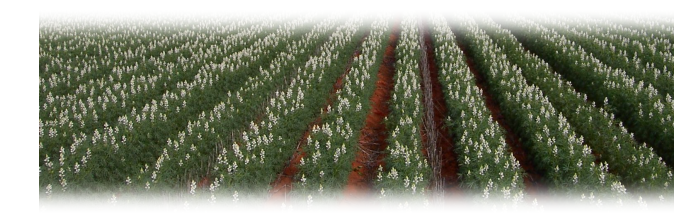
\includegraphics[width = 8cm]{lupin}
\end{frame}

%%%%%%%%%%%%%%%%%%%%%%%%%%%%%%%%%%%%%%%%%%%%%%%%%%%%%%%%%%%%%%%%%%%%%%%%%%%%%%%%%%%%%%%%%%%%%%%%%%%
% Slide
%%%%%%%%%%%%%%%%%%%%%%%%%%%%%%%%%%%%%%%%%%%%%%%%%%%%%%%%%%%%%%%%%%%%%%%%%%%%%%%%%%%%%%%%%%%%%%%%%%%
\begin{frame}\frametitle{Experimental Layout}

\begin{center}
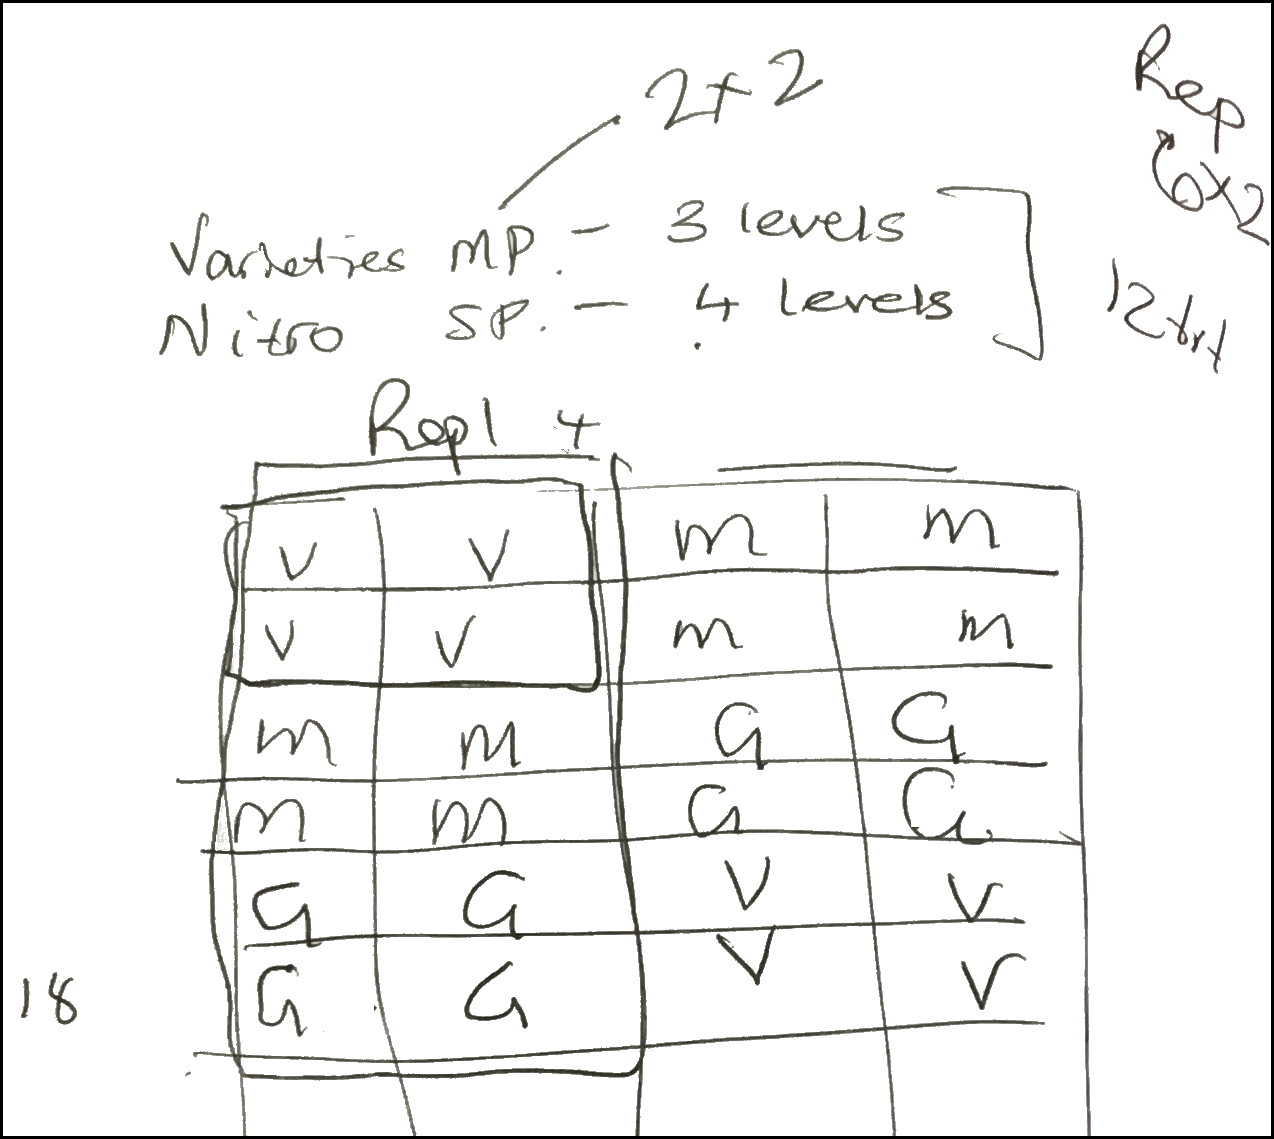
\includegraphics[height = 0.7\textheight]{exptlayout.png}
\end{center}
\flushright

\includegraphics[height = 0.3cm]{yourturn}
\end{frame}


%%%%%%%%%%%%%%%%%%%%%%%%%%%%%%%%%%%%%%%%%%%%%%%%%%%%%%%%%%%%%%%%%%%%%%%%%%%%%%%%%%%%%%%%%%%%%%%%%%%
% Slide
%%%%%%%%%%%%%%%%%%%%%%%%%%%%%%%%%%%%%%%%%%%%%%%%%%%%%%%%%%%%%%%%%%%%%%%%%%%%%%%%%%%%%%%%%%%%%%%%%%%
\begin{frame}\frametitle{Latin Square - Linear Model}
The linear model that is fit can be symbolically written as:
\begin{eqnarray*}
	\texttt{Response variable}&:& \texttt{Dry Matter} \\
	\texttt{Structural component}&:& \texttt{Row, Column}\\
	\texttt{Explanatory component}&:& \texttt{Soil Type}\\
	\texttt{Residual}&:& \texttt{Assume Independence}
\end{eqnarray*}
\end{frame}

%%%%%%%%%%%%%%%%%%%%%%%%%%%%%%%%%%%%%%%%%%%%%%%%%%%%%%%%%%%%%%%%%%%%%%%%%%%%%%%%%%%%%%%%%%%%%%%%%%%
% Slide
%%%%%%%%%%%%%%%%%%%%%%%%%%%%%%%%%%%%%%%%%%%%%%%%%%%%%%%%%%%%%%%%%%%%%%%%%%%%%%%%%%%%%%%%%%%%%%%%%%%
\begin{frame}\frametitle{Example 4}
\begin{enumerate}
\item The null hypothesis is that all the soil types will have the same Dry Matter, that is:
\begin{align*}
& H_0: \texttt{The lupin dry matter is not dependent on the soil type}\\
& H_1:\texttt{The lupin dry matter is not dependent on the soil type}\\
\end{align*}
\item A Latin square design has been used. \\
\item The treatments are the soil types.\\
\item The experimental unit is the pot, as the soil types have been randomised to the pots.\\
\item The observational unit is also the pot.\\
\item The experiment was conducted in the glasshouse in a rectangular array of rows and columns.\\
\end{enumerate}
\end{frame}


%%%%%%%%%%%%%%%%%%%%%%%%%%%%%%%%%%%%%%%%%%%%%%%%%%%%%%%%%%%%%%%%%%%%%%%%%%%%%%%%%%%%%%%%%%%%%%%%%%%
% Slide
%%%%%%%%%%%%%%%%%%%%%%%%%%%%%%%%%%%%%%%%%%%%%%%%%%%%%%%%%%%%%%%%%%%%%%%%%%%%%%%%%%%%%%%%%%%%%%%%%%%

\begin{frame}\frametitle{Looking at the multiple comparison test}
At the family 5\% significance level:
\begin{itemize}
\item S1 and S4 are significantly different
\item S2 and S3 are significantly different
\item S3 is not significantly different to S1 but significantly different
      from both S2 or S4
\item S4 is not significantly different to S2 but significantly different
      from S3
\end{itemize}
\end{frame}

\end{document}
